\documentclass[11pt,a4paper]{article}
\usepackage[margin=2.2cm]{geometry}
\usepackage[T1]{fontenc}
\usepackage{lmodern}
\usepackage{graphicx,booktabs,tabularx,longtable,float,amsmath,array}
\usepackage[font=small,labelfont=bf]{caption}
\usepackage[authoryear,round]{natbib}
\usepackage[hidelinks]{hyperref}
\usepackage{setspace}
\setstretch{1.05}
\setlength{\parskip}{0.4em}
\setlength{\parindent}{0pt}
\renewcommand{\topfraction}{0.9}\renewcommand{\bottomfraction}{0.8}
\renewcommand{\textfraction}{0.07}\renewcommand{\floatpagefraction}{0.85}
\setcounter{topnumber}{3}\setcounter{bottomnumber}{2}\setcounter{totalnumber}{5}
\renewcommand{\arraystretch}{1.12}
\newcolumntype{Y}{>{\raggedright\arraybackslash}X}
\newcolumntype{C}{>{\centering\arraybackslash}X}
\graphicspath{{figures/}}
\title{\textbf{FX Carry Trade: Portfolio Construction, Crash Risk and Factor Analysis}\\[0.3em]
\large Eight G10 currencies against the US dollar, August 2016 -- August 2026}
\author{Partha Gunturu\\ \small M.Sc. Quantitative Finance, Ahmedabad University \quad Topic 9: Carry \& Macro Strategies}
\date{November 2026}
\begin{document}
\maketitle

\begin{abstract}
\noindent We test a monthly long-short carry strategy on eight major currencies against the US dollar (EUR, GBP, JPY, CHF,
NOK, AUD, NZD, CAD) using Bloomberg spot and one-month forward data, September 2016 to July 2026 (119 months). Buying the
three highest-rate and selling the three lowest-rate currencies made 2.92\% a year after costs, with a Sharpe ratio of 0.44.
The profit came almost entirely from the interest-rate gap; exchange-rate moves added nothing, against uncovered interest
parity (UIP). Returns are skewed to the downside, and the five worst months all match global shocks (COVID-19, the Fed hikes
of 2018 and 2022, Omicron and the 2024 yen-carry unwind). Carry does well in calm markets, loses in crises and moves with
equities; after controlling for equity and volatility risk its extra return is close to zero. A three-month momentum filter
made results worse. Carry is a reward for crash risk, not a free lunch.
\end{abstract}

\section{Introduction}
A carry trade borrows in a low-rate currency and invests in a high-rate one. Under uncovered interest parity (UIP) the
high-rate currency should fall by the rate gap, leaving no profit. In practice it usually does not fall enough, so carry
makes money over long periods \citep{fama1984,engel1996,lrv2011}. The risk is sudden crashes, such as the yen-carry unwind
of 2008: carry goes ``up the stairs and down the elevator'' \citep{bnp2009}.

The period 2016--2026 is a good test. It covers the Fed hikes of 2017--18, the COVID-19 crash, the 2022--23 global rate
rises, the end of negative rates in Japan and the August 2024 yen unwind, the April 2025 tariff shock and the 2026 oil
shock. We ask: (1) Does carry earn a positive Sharpe ratio, and how does it vary between calm and stressed markets?
(2) Does UIP hold, and where does the return come from? (3) How large is crash risk, and which events caused it?
(4) Is carry a risk factor linked to equities and the VIX? (5) Does a momentum filter help?

\section{Literature Review}
\textbf{UIP and its failure.} Under UIP, the forward rate should predict the future spot rate. \citet{fama1984} regressed
spot changes on the forward premium and found slopes below one and often negative (the \emph{forward premium puzzle});
\citet{hansenhodrick1980} and \citet{engel1996} confirm this across currencies. Since 2008, covered-parity gaps also affect
JPY and CHF forwards \citep{dtv2018}.

\textbf{Carry as a risk premium.} \citet{lrv2011} show that a dollar factor (DOL) and a carry factor (HML\textsubscript{FX})
explain most currency returns, with high-rate currencies loading positively on carry. \citet{msss2012a} find carry loses
when global FX volatility rises, while JPY and CHF hedge. \citet{koijen2018} find carry across asset classes, and
\citet{burnside2012} reviews the risk-based explanations.

\textbf{Crash risk.} \citet{bnp2009} show carry is negatively skewed and crashes when the VIX rises and traders unwind.
\citet{jurek2014} finds option hedges remove part of the return; \citet{burnside2011} point to rare unseen disasters;
\citet{dhl2017} document large drawdowns. \citet{msss2012b} find momentum weak among major currencies. The BIS
\citep{bis2025,bis2024} documents the size of FX funding markets and links August 2024 to the unwinding of yen carry.

\section{Data and Method}
\subsection{Bloomberg data}
\textbf{GP}: daily spot rates for EURUSD, GBPUSD, AUDUSD, NZDUSD, USDJPY, USDCHF, USDCAD, USDNOK, plus the S\&P 500 and VIX
(18 Aug 2016 -- 17 Aug 2026, 2,608 days). \textbf{FRD}: one-month forward points (forward = spot + points/10,000; /100 for
JPY). \textbf{WIRP}: implied central-bank paths on 17 Aug 2026, used as a forward-looking check only. \textbf{FXIP}: forward
points grid; positioning data were not available. All rates are quoted as USD per foreign currency, so a positive return
means the currency rose against USD. We use month-end data and drop the partial August 2026, leaving 119 holding months.

\begin{table}[!htbp]\centering\small
\caption{The eight currencies against the US dollar, September 2016 -- July 2026}\label{tab:ccy}
\begin{tabularx}{\textwidth}{lCCCCCC}
\toprule Currency & Rate gap vs USD (\% p.a.) & Spot change (\% p.a.) & Carry return (\% p.a.) & Volatility (\% p.a.) & Months long (\%) & Months short (\%) \\ \midrule
EUR & $-$1.92 & +0.57 & $-$1.36 & 6.92 & 0 & 98 \\
GBP & $-$0.68 & +0.57 & $-$0.11 & 7.90 & 44 & 1 \\
JPY & $-$2.86 & $-$3.82 & $-$6.67 & 9.03 & 0 & 99 \\
CHF & $-$3.02 & +2.27 & $-$0.76 & 7.47 & 0 & 100 \\
NOK & $-$0.59 & $-$0.61 & $-$1.20 & 11.78 & 53 & 0 \\
AUD & $-$0.40 & $-$0.23 & $-$0.62 & 9.68 & 53 & 0 \\
NZD & $-$0.13 & $-$1.54 & $-$1.67 & 10.72 & 82 & 0 \\
CAD & $-$0.64 & $-$0.47 & $-$1.11 & 6.47 & 68 & 2 \\
\bottomrule\end{tabularx}
\par\vspace{0.3em}\footnotesize\emph{Rate gap = one-month forward discount, annualised (roughly foreign rate minus US rate). Carry return = return from holding a one-month forward and rolling it each month.}
\end{table}

Over this period the US dollar paid more than every other currency
(Table~\ref{tab:ccy}). CHF ($-$3.0 points), JPY ($-$2.9) and EUR ($-$1.9) were the cheapest to borrow. Because the strategy
ranks currencies against each other, the bought basket still paid 2.48 points more than the sold basket on average.

\subsection{Portfolio construction}
At each month-end the carry signal is the one-month forward discount:
\begin{equation}
c_{i,t} = \frac{S_{i,t}}{F_{i,t}} - 1 \;\approx\; \frac{i_{\text{foreign},t} - i_{\text{USD},t}}{12}
\end{equation}
We buy the top three and sell the bottom three (one third each) and hold to the next month-end. The return of a forward
position splits into a spot part and a carry part:
\begin{equation}
x_{i,t+1} = \frac{S_{i,t+1}}{F_{i,t}} - 1 \;=\; \underbrace{\left(\frac{S_{i,t+1}}{S_{i,t}} - 1\right)}_{\text{spot}}
\;+\; \underbrace{c_{i,t}}_{\text{carry}} \;+\; \text{cross term}
\end{equation}
Costs are 5 bp per unit of turnover. Benchmarks: a \textbf{dollar basket (DOL)} holding all eight currencies, and
\textbf{static carry}, which keeps the first month's positions throughout.

\subsection{Measures}
Sharpe = mean $\times12$ / volatility $\times\sqrt{12}$; Sortino uses downside volatility; Calmar = growth rate / maximum
drawdown; tail ratio = average of the worst 5\% of months / average of the best 5\%. UIP is tested with the
\citet{fama1984} regression $\Delta s_{i,t+1} = \alpha_i + \beta_i (f_{i,t} - s_{i,t}) + \varepsilon$, where UIP means
$\beta = 1$. Regimes split months by the VIX median (17.5) and flag crisis months (VIX $\geq$ 30). The momentum filter keeps a
long only if the currency rose over three months and a short only if it fell. Standard errors are Newey--West (3 lags).
Code: \texttt{src/carry\_project.py}.

\section{The Long and Short Positions}
\textbf{Short side.} The funding basket barely changed: CHF was sold in 100\% of months, JPY in 99\% and EUR in 98\%. All
three central banks kept rates at or below zero for most of the period. The only swaps were GBP for JPY in December 2021,
and CAD for EUR from June 2026 after the ECB hiked.

\textbf{Long side.} The long basket rotated as central banks diverged:
\begin{itemize}\setlength{\itemsep}{0pt}
\item \textbf{2016--2019: AUD, NZD, CAD} --- highest rates at the start; held two years (July 2017 -- June 2019).
\item \textbf{2019--2022: NOK, NZD, CAD} --- frequent changes as COVID cuts squeezed all rate gaps.
\item \textbf{2023 -- mid 2024: GBP, NZD, CAD} --- the Bank of England hiked to 5.25\%; held 19 months.
\item \textbf{Dec 2024 -- 2026: AUD, GBP, NOK} --- the RBA and Norges Bank kept rates high and hiked again in 2026.
\end{itemize}
Every position is against USD, so the dollar legs largely cancel and the portfolio is in effect long crosses such as NZD/JPY,
CAD/CHF and GBP/EUR (Tables~\ref{tab:pairs} and~\ref{tab:history}).

\begin{table}[!htbp]\centering\small
\caption{How each currency position is traded, and how often it was used}\label{tab:pairs}
\begin{tabularx}{\textwidth}{llCYCY}
\toprule Currency & Bloomberg pair & Months long (\%) & Trade when long & Months short (\%) & Trade when short \\ \midrule
NZD & NZDUSD & 82.4 & Buy NZDUSD & 0.0 & Sell NZDUSD \\
CAD & USDCAD & 68.1 & Sell USDCAD & 1.7 & Buy USDCAD \\
AUD & AUDUSD & 52.9 & Buy AUDUSD & 0.0 & Sell AUDUSD \\
NOK & USDNOK & 52.9 & Sell USDNOK & 0.0 & Buy USDNOK \\
GBP & GBPUSD & 43.7 & Buy GBPUSD & 0.8 & Sell GBPUSD \\
EUR & EURUSD & 0.0 & Buy EURUSD & 98.3 & Sell EURUSD \\
JPY & USDJPY & 0.0 & Sell USDJPY & 99.2 & Buy USDJPY \\
CHF & USDCHF & 0.0 & Sell USDCHF & 100.0 & Buy USDCHF \\
\bottomrule\end{tabularx}
\par\vspace{0.3em}\footnotesize\emph{Long a currency = buy it against USD; short = sell it against USD. For pairs quoted as USD per currency (USDJPY, USDCHF, USDCAD, USDNOK) the trade direction is reversed.}
\end{table}

{\small
\begin{longtable}{llcp{3.6cm}p{3.6cm}c}
\caption{Position history: every period in which the long and short baskets stayed the same}\label{tab:history}\\
\toprule From & To & Months & Long (high-rate) & Short (funding) & Return (\%) \\ \midrule \endfirsthead
\toprule From & To & Months & Long (high-rate) & Short (funding) & Return (\%) \\ \midrule \endhead
\bottomrule \endlastfoot
2016-09 & 2017-02 & 6 & AUD, NOK, NZD & CHF, EUR, JPY & +6.85 \\
2017-03 & 2017-03 & 1 & AUD, CAD, NZD & CHF, EUR, JPY & $-$1.59 \\
2017-04 & 2017-06 & 3 & AUD, NOK, NZD & CHF, EUR, JPY & $-$0.26 \\
2017-07 & 2019-06 & 24 & AUD, CAD, NZD & CHF, EUR, JPY & $-$2.14 \\
2019-07 & 2020-03 & 9 & CAD, NOK, NZD & CHF, EUR, JPY & $-$10.33 \\
2020-04 & 2020-04 & 1 & AUD, NOK, NZD & CHF, EUR, JPY & +3.94 \\
2020-05 & 2020-06 & 2 & AUD, CAD, NZD & CHF, EUR, JPY & +3.53 \\
2020-07 & 2020-07 & 1 & CAD, NOK, NZD & CHF, EUR, JPY & $-$0.26 \\
2020-08 & 2020-09 & 2 & AUD, CAD, NZD & CHF, EUR, JPY & +0.73 \\
2020-10 & 2020-10 & 1 & AUD, NOK, NZD & CHF, EUR, JPY & $-$1.50 \\
2020-11 & 2021-05 & 7 & CAD, NOK, NZD & CHF, EUR, JPY & +11.20 \\
2021-06 & 2021-08 & 3 & CAD, GBP, NZD & CHF, EUR, JPY & $-$1.58 \\
2021-09 & 2021-11 & 3 & CAD, NOK, NZD & CHF, EUR, JPY & $-$0.16 \\
2021-12 & 2021-12 & 1 & CAD, NOK, NZD & CHF, EUR, GBP & +0.43 \\
2022-01 & 2022-02 & 2 & GBP, NOK, NZD & CHF, EUR, JPY & +0.22 \\
2022-03 & 2022-03 & 1 & CAD, NOK, NZD & CHF, EUR, JPY & +3.99 \\
2022-04 & 2022-04 & 1 & GBP, NOK, NZD & CHF, EUR, JPY & $-$0.46 \\
2022-05 & 2022-05 & 1 & CAD, GBP, NOK & CHF, EUR, JPY & $-$0.56 \\
2022-06 & 2022-06 & 1 & CAD, GBP, NZD & CHF, EUR, JPY & $-$0.58 \\
2022-07 & 2022-09 & 3 & AUD, CAD, NZD & CHF, EUR, JPY & $-$2.33 \\
2022-10 & 2022-10 & 1 & CAD, NOK, NZD & CHF, EUR, JPY & +4.65 \\
2022-11 & 2022-11 & 1 & CAD, GBP, NZD & CHF, EUR, JPY & $-$1.05 \\
2022-12 & 2022-12 & 1 & CAD, NOK, NZD & CHF, EUR, JPY & $-$3.11 \\
2023-01 & 2024-07 & 19 & CAD, GBP, NZD & CHF, EUR, JPY & +7.10 \\
2024-08 & 2024-11 & 4 & GBP, NOK, NZD & CHF, EUR, JPY & +1.16 \\
2024-12 & 2026-05 & 18 & AUD, GBP, NOK & CHF, EUR, JPY & +11.16 \\
2026-06 & 2026-07 & 2 & AUD, GBP, NOK & CAD, CHF, JPY & +0.35 \\
\end{longtable}
\vspace{-0.6em}\par\footnotesize\emph{Return = compounded net return of the portfolio over the period.}\par
}

The two longest holding periods were the most profitable ($+$7.1\% and $+$11.2\%); the worst was
July 2019 -- March 2020 ($-$10.3\%), long NOK, NZD and CAD into COVID and the oil collapse.

\section{Results: Portfolio Performance}
\begin{table}[!htbp]\centering\small
\caption{Performance summary, monthly returns, September 2016 -- July 2026 (119 months)}\label{tab:perf}
\begin{tabularx}{\textwidth}{lCCCCC}
\toprule  & Carry (net) & Carry (gross) & Static carry & Dollar basket & S\&P 500 \\ \midrule
Average return (\% p.a.) & 2.92 & 2.97 & 1.76 & $-$1.69 & 13.73 \\
Growth rate, CAGR (\%) & 2.73 & 2.78 & 1.49 & $-$1.93 & 13.30 \\
Volatility (\% p.a.) & 6.61 & 6.61 & 7.53 & 7.26 & 15.40 \\
Sharpe ratio & 0.44 & 0.45 & 0.23 & $-$0.23 & 0.89 \\
Sortino ratio & 0.64 & 0.65 & 0.33 & $-$0.31 & 1.42 \\
Maximum drawdown (\%) & $-$14.04 & $-$14.03 & $-$17.13 & $-$25.67 & $-$24.77 \\
Calmar ratio & 0.20 & 0.20 & 0.09 & $-$0.07 & 0.54 \\
Skewness & $-$0.54 & $-$0.54 & $-$0.51 & 0.03 & $-$0.43 \\
Excess kurtosis & 0.99 & 1.00 & 0.47 & $-$0.34 & 0.62 \\
Worst month (\%) & $-$6.41 & $-$6.41 & $-$6.84 & $-$5.25 & $-$12.51 \\
Best month (\%) & 4.65 & 4.67 & 4.85 & 5.55 & 12.68 \\
Positive months (\%) & 58.8 & 58.8 & 59.7 & 43.7 & 67.2 \\
Tail ratio & 1.08 & 1.08 & 1.22 & 1.04 & 0.95 \\
t-statistic (mean = 0) & 1.79 & 1.83 & 0.92 & $-$0.82 & 3.45 \\
\bottomrule\end{tabularx}
\par\vspace{0.3em}\footnotesize\emph{Net = after 5 bp per unit of turnover. Static carry keeps the September 2016 positions. Dollar basket = equal weights in all eight currencies against USD. S\&P 500 = price return.}
\end{table}

\textbf{Main result.} Carry made 2.92\% a year after costs, with 6.61\% volatility, Sharpe 0.44 and Sortino 0.64
(Table~\ref{tab:perf}). It was positive in 59\% of months, but the t-statistic of 1.79 is significant only at 10\%. The
maximum drawdown was 14.0\% (August 2017 -- March 2020, recovered March 2021). Costs are negligible: only 8\% of the
portfolio is traded per month.

\textbf{Against buy-and-hold.} Rebalancing added value. Static carry made 1.76\% (Sharpe 0.23) because it held NZD and AUD
after their rates fell. The dollar basket lost 1.69\% (Sharpe $-$0.23) against a strong, high-yielding dollar. The S\&P 500
made 13.7\%, but carry rises and falls with it (Section 8), so it does not diversify equities.

\begin{figure}[!htbp]\centering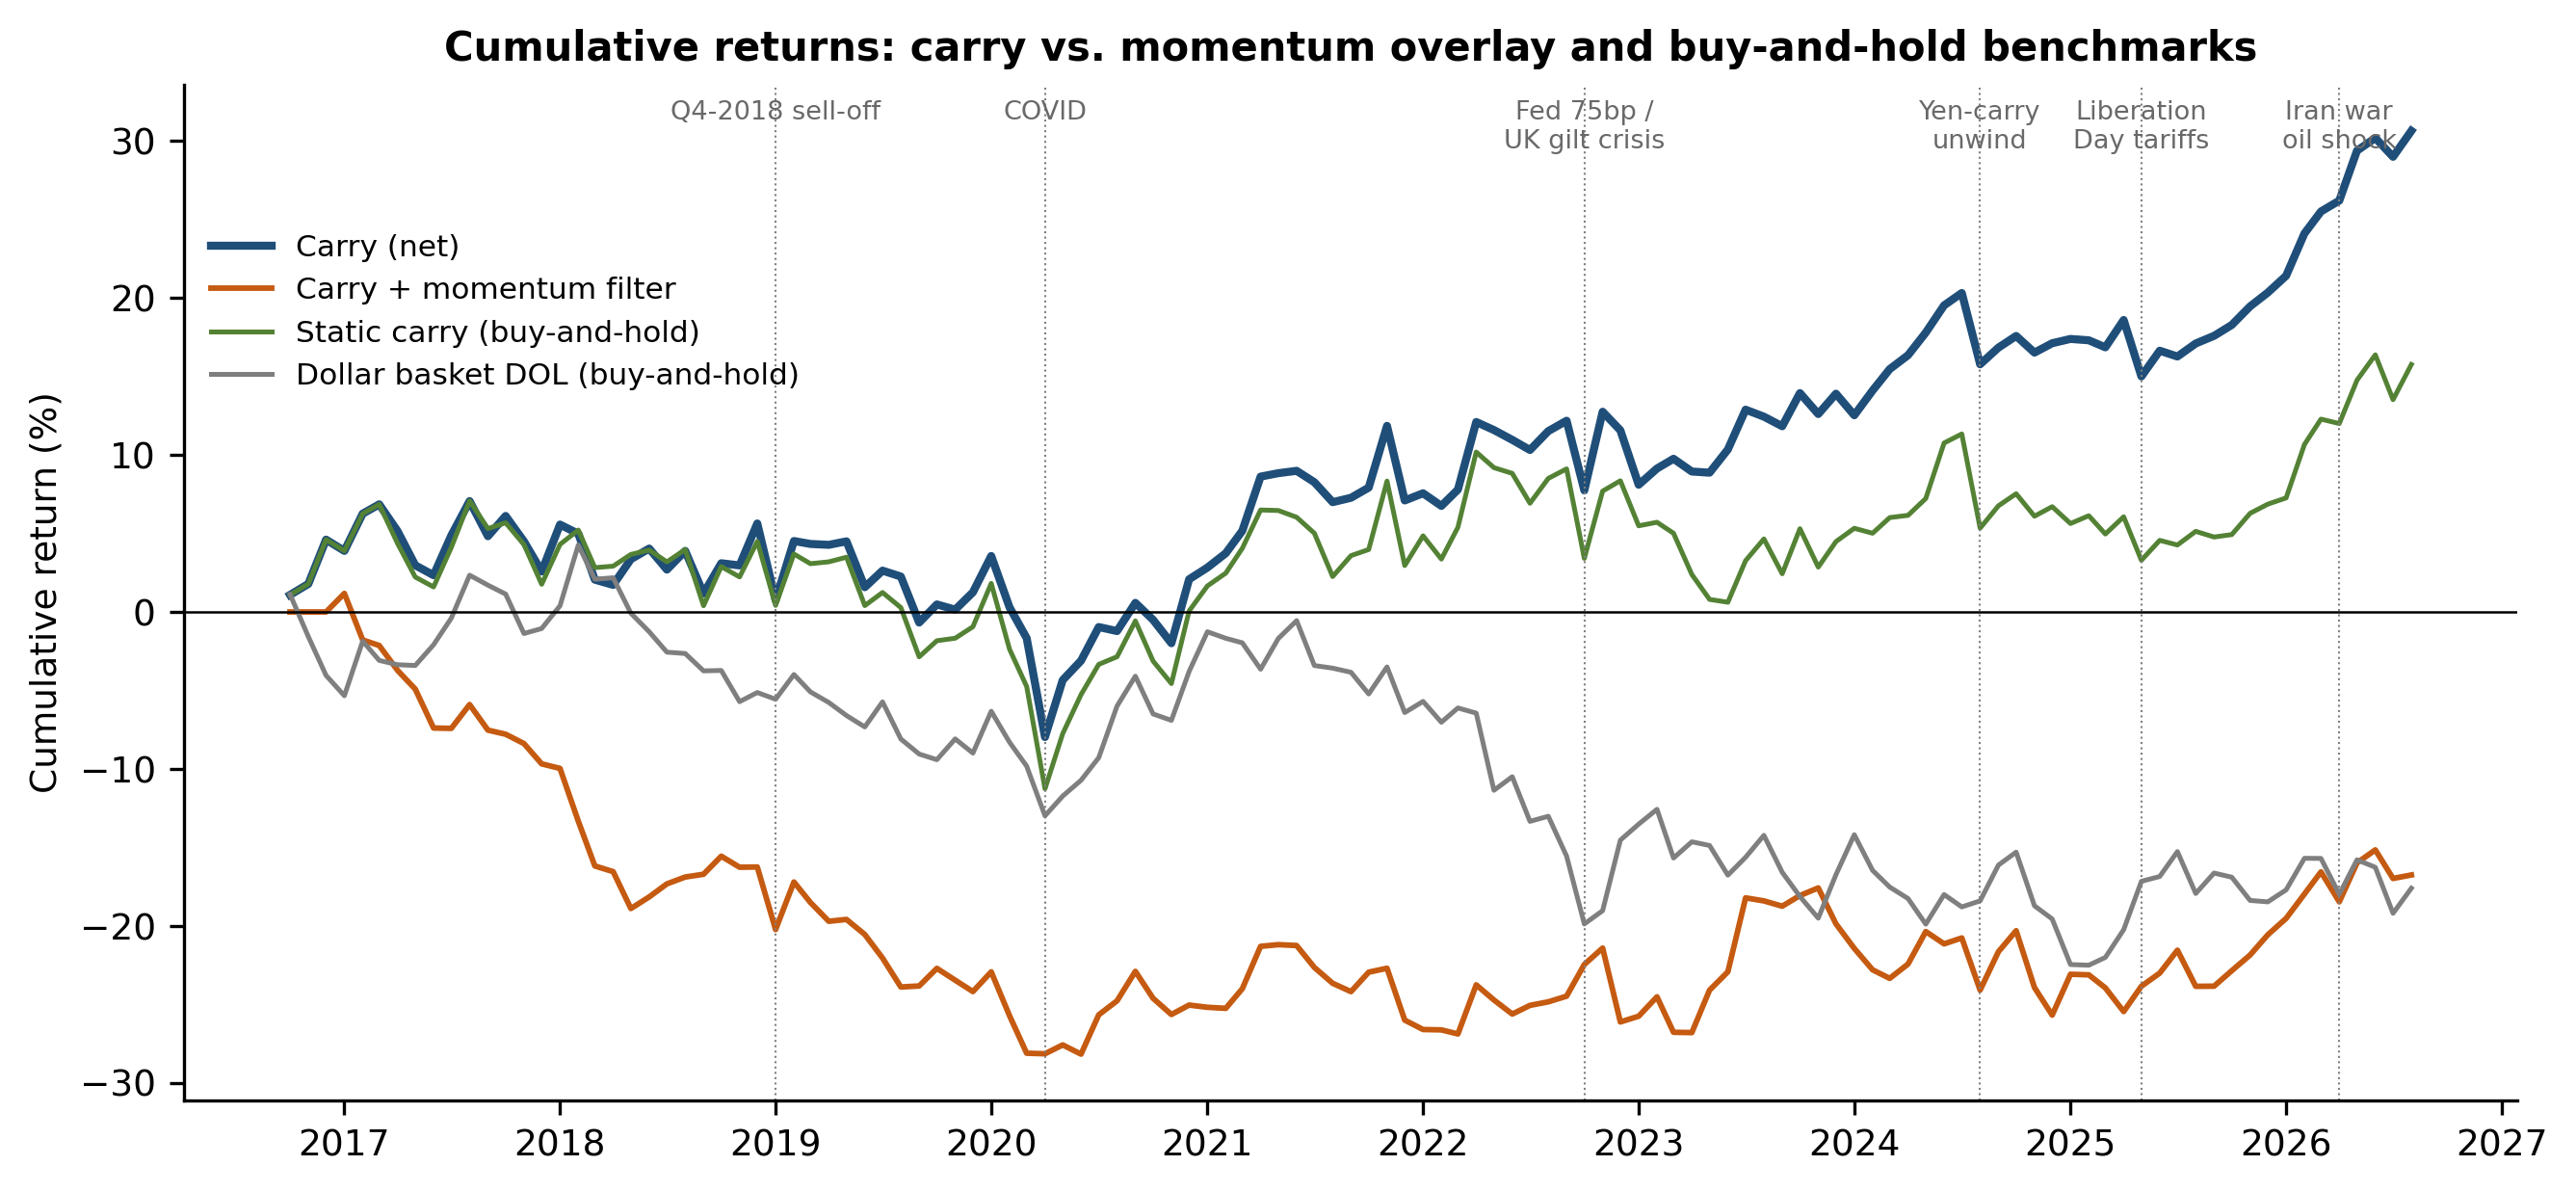
\includegraphics[width=0.78\textwidth]{figures/F01_cumulative_returns.png}\caption{Cumulative returns of carry, carry with the momentum filter, and the two buy-and-hold portfolios. Dotted lines mark the main market shocks.}\label{fig:cum}\end{figure}

\begin{table}[!htbp]\centering\small
\caption{Where the return comes from}\label{tab:dec}
\begin{tabularx}{\textwidth}{p{5.5cm}CCC}
\toprule Part of return & Average per month (\%) & Per year (\%) & t-statistic \\ \midrule
Spot (FX) component & 0.041 & 0.49 & 0.30 \\
Carry (forward discount) component & 0.206 & 2.48 & 14.25 \\
Cross term & 0.000 & 0.00 & 0.18 \\
Gross excess return & 0.247 & 2.97 & 1.83 \\
Transaction costs & 0.004 & 0.05 & 4.44 \\
Net return & 0.243 & 2.92 & 1.79 \\
\bottomrule\end{tabularx}
\end{table}

\textbf{Source of return.} The carry part gave 2.48\% a year (t = 14.2); the spot part gave 0.49\% (t = 0.30), i.e.
nothing (Table~\ref{tab:dec}, Figure~\ref{fig:dec}). The strategy earned the rate gap and exchange rates did not take it away.

\begin{figure}[!htbp]\centering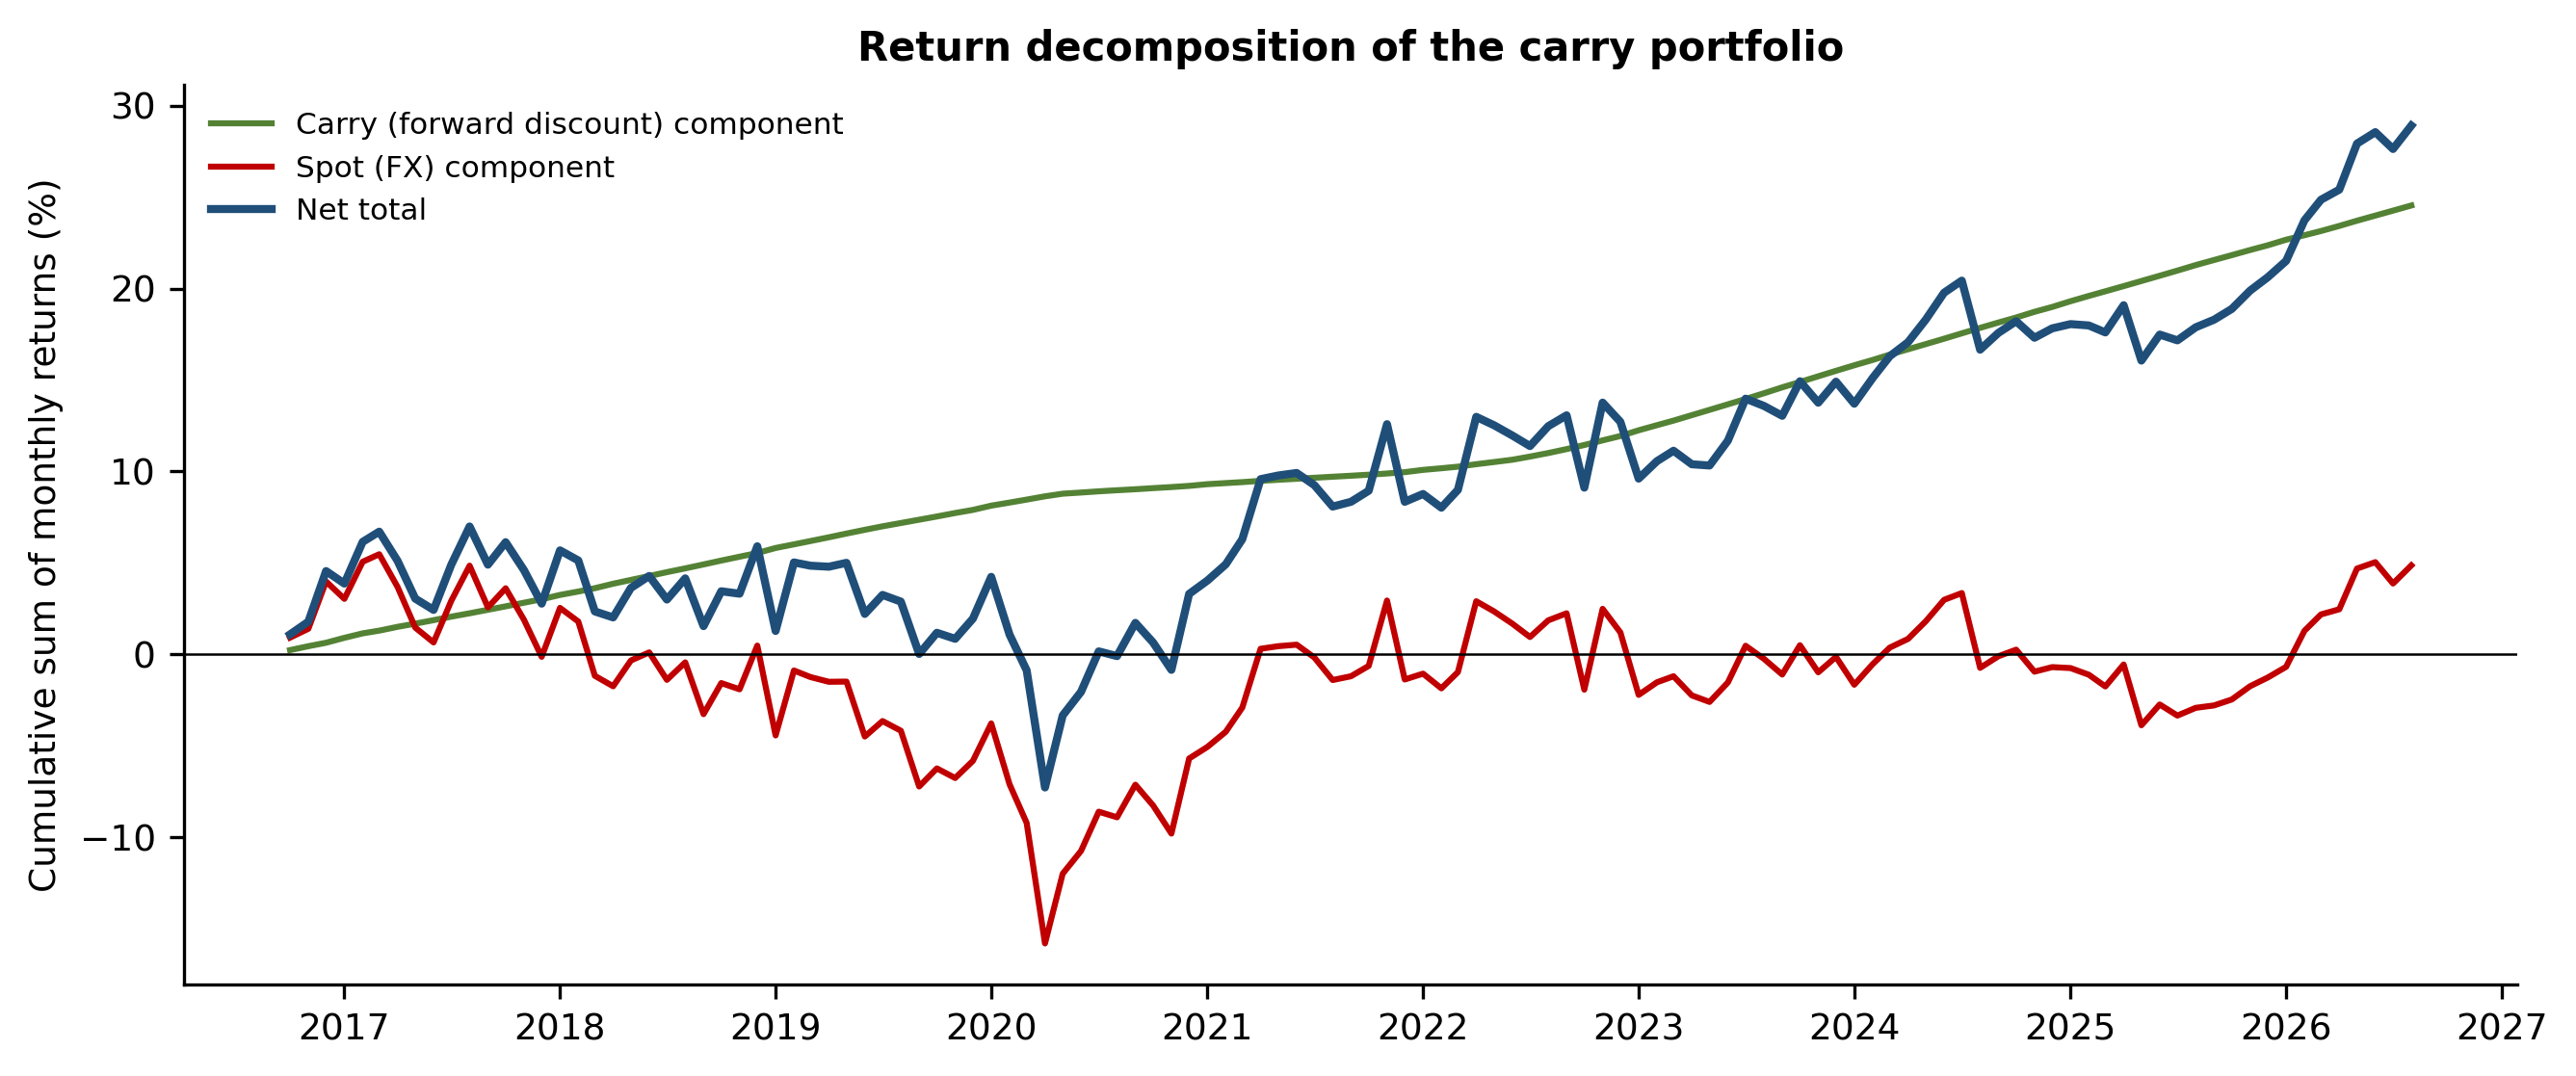
\includegraphics[width=0.75\textwidth]{figures/F02_return_decomposition.png}\caption{Cumulative carry part and spot part of the portfolio return.}\label{fig:dec}\end{figure}

\begin{table}[!htbp]\centering\small
\caption{Performance by sub-period (net)}\label{tab:sub}
\begin{tabularx}{\textwidth}{lCCCCCC}
\toprule Period & Months & Return (\% p.a.) & Volatility (\% p.a.) & Sharpe & Max drawdown (\%) & t-stat \\ \midrule
2016-09 to 2019-12 & 40 & 1.27 & 6.68 & 0.19 & $-$7.23 & 0.51 \\
2020-01 to 2022-12 & 36 & 1.79 & 8.61 & 0.21 & $-$8.24 & 0.43 \\
2023-01 to end & 43 & 5.39 & 4.34 & 1.24 & $-$4.42 & 2.76 \\
\bottomrule\end{tabularx}
\end{table}

\textbf{Over time.} Before 2023 the Sharpe ratio was about 0.2 (Table~\ref{tab:sub}, Figures~\ref{fig:annual}
and~\ref{fig:rs}): 2018 lost 4.6\% on Fed hikes and the US--China trade war, and 2020 was slightly negative. From 2023 carry
made 5.39\% a year (Sharpe 1.24) as Japan and Switzerland stayed near zero while the UK, Norway and Australia kept rates
high. January--July 2026 made 7.6\%.

\begin{figure}[!htbp]\centering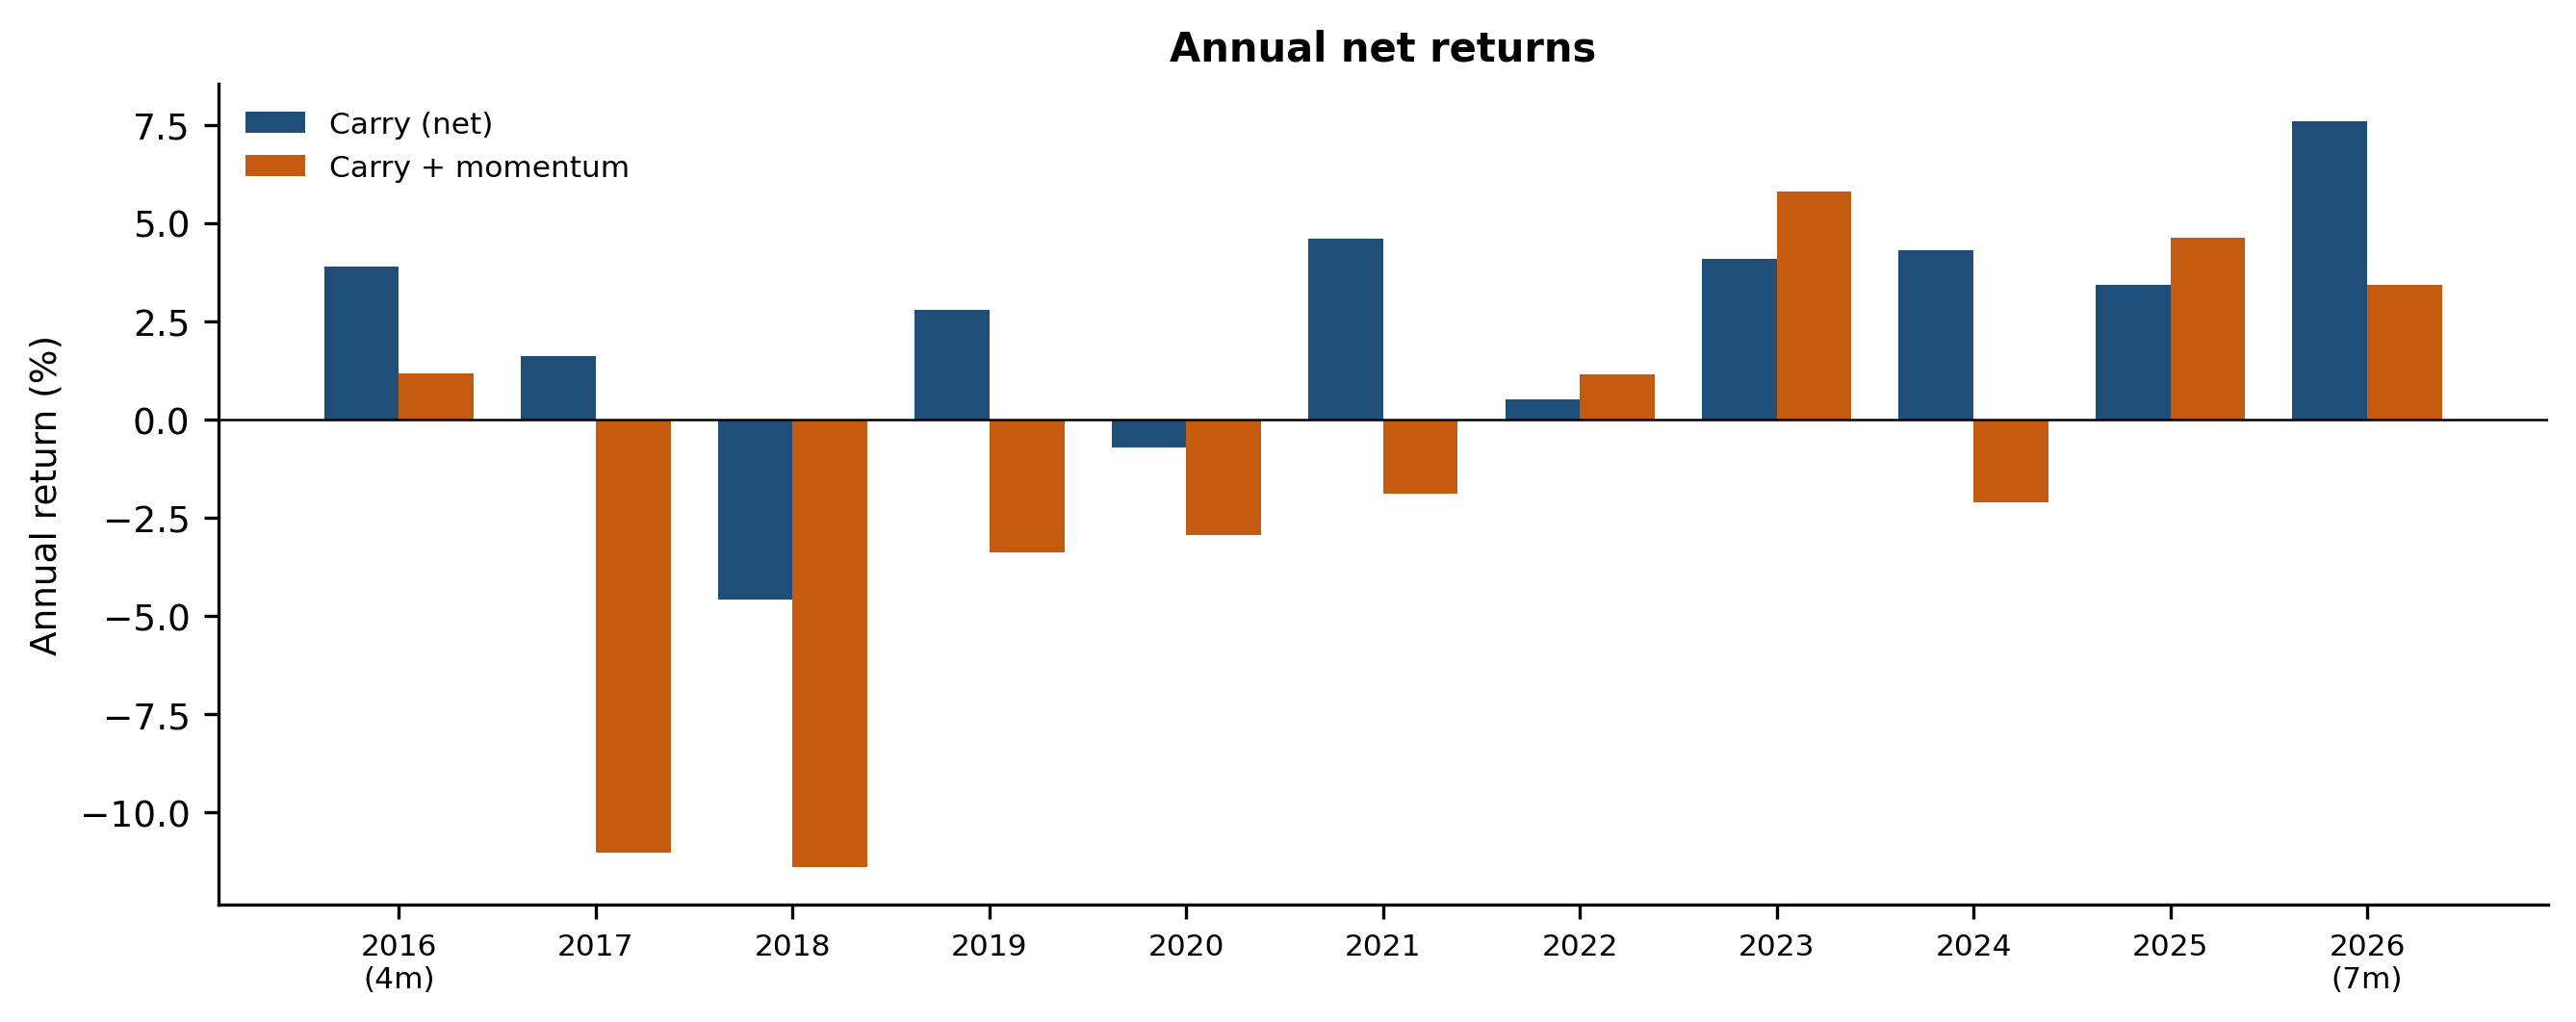
\includegraphics[width=0.7\textwidth]{figures/F03_annual_returns.png}\caption{Yearly net returns of carry and carry with the momentum filter (2016: Sep--Dec; 2026: Jan--Jul).}\label{fig:annual}\end{figure}

\begin{figure}[!htbp]\centering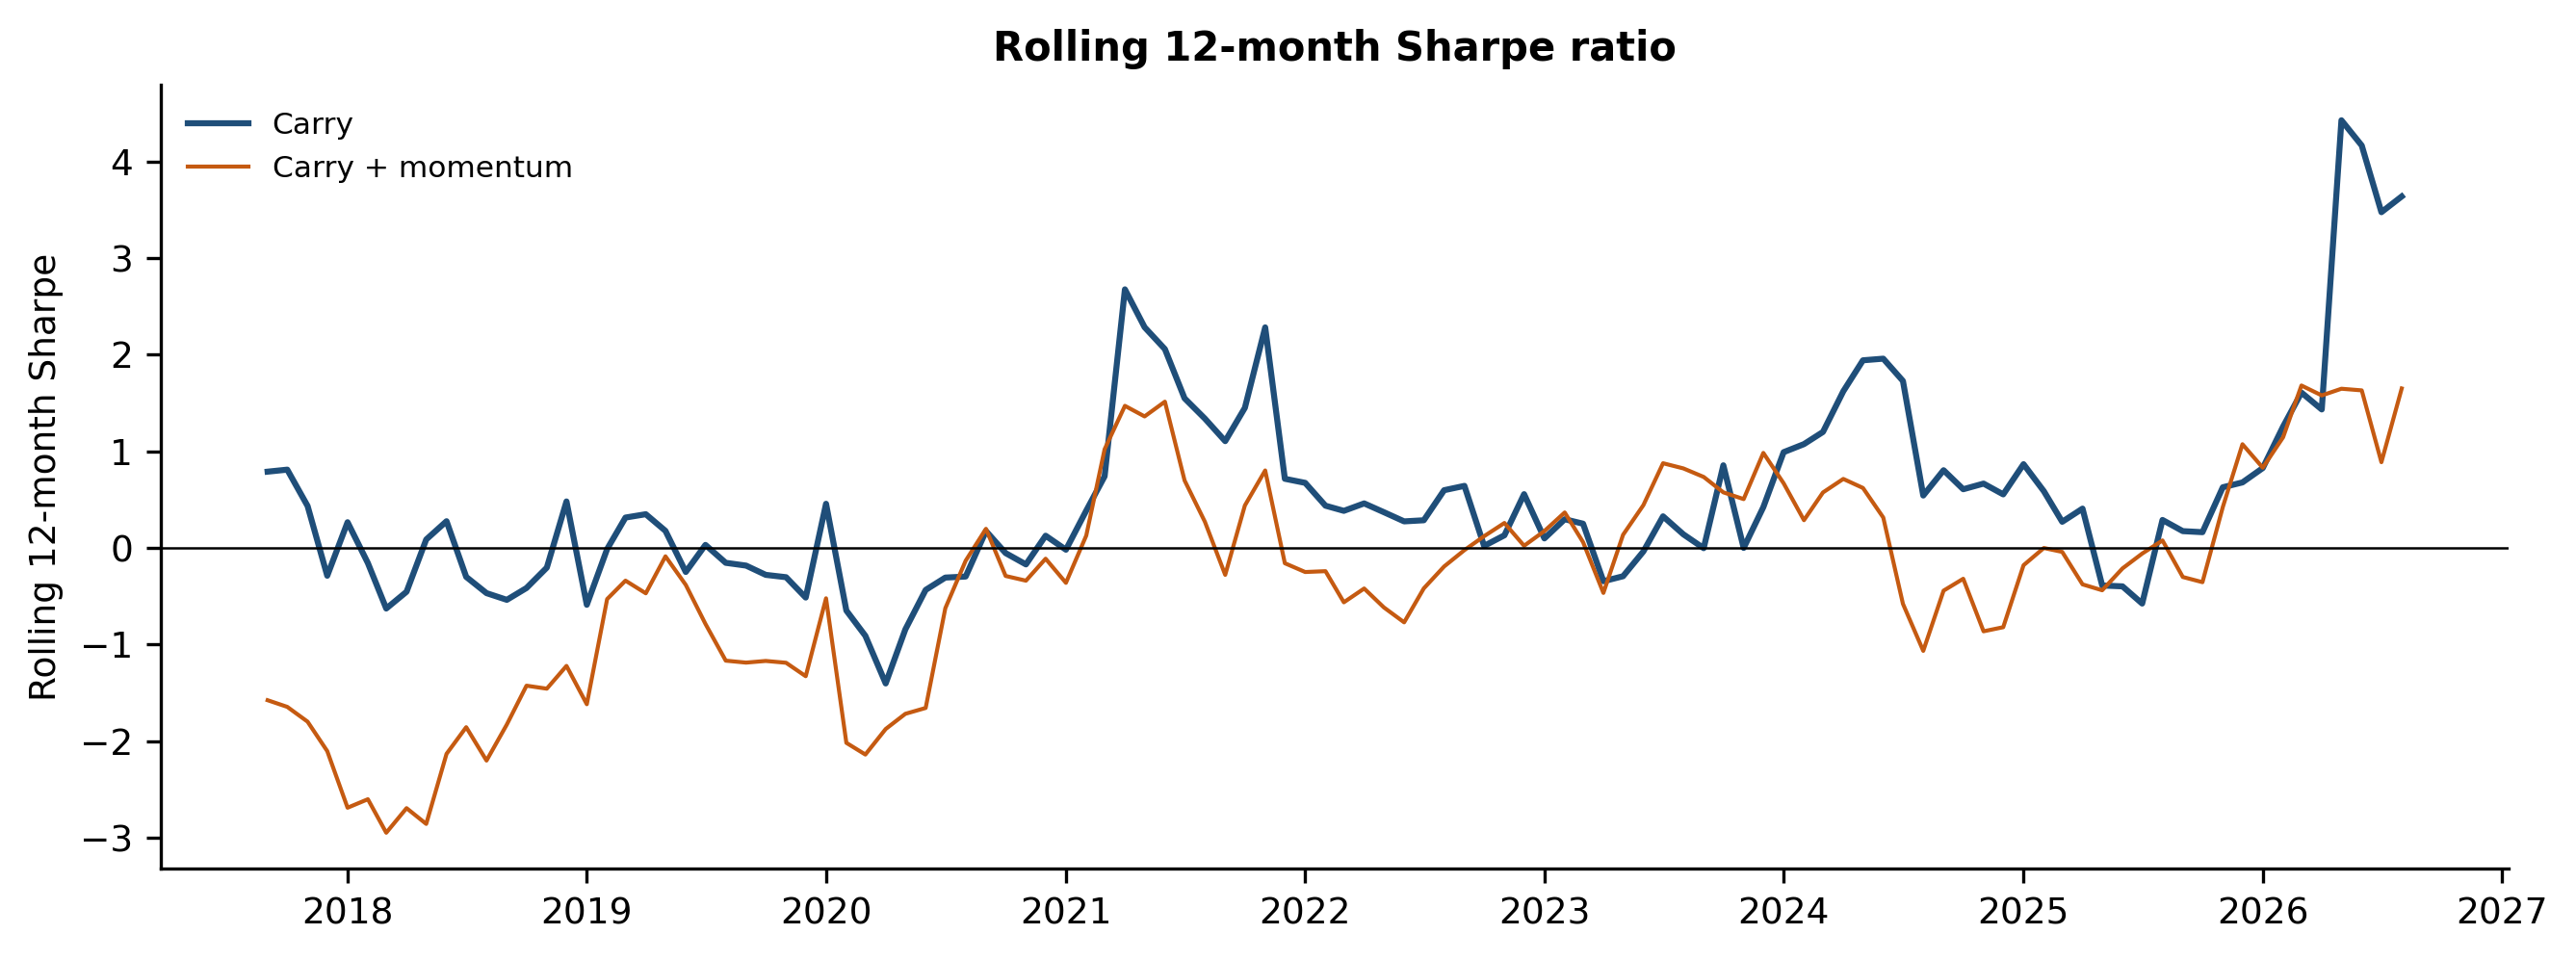
\includegraphics[width=0.7\textwidth]{figures/F04_rolling_sharpe.png}\caption{Rolling 12-month Sharpe ratio.}\label{fig:rs}\end{figure}

\begin{table}[!htbp]\centering\small
\caption{Carry performance in calm and stressed markets}\label{tab:reg}
\begin{tabularx}{\textwidth}{p{4.0cm}CCCCCC}
\toprule Market regime & Months & Return (\% p.a.) & Volatility (\% p.a.) & Sharpe & Worst month (\%) & Positive months (\%) \\ \midrule
Low VIX (below median 17.5) & 59 & 3.37 & 5.26 & 0.64 & $-$3.78 & 61.0 \\
High VIX (above median) & 60 & 2.47 & 7.75 & 0.32 & $-$6.41 & 56.7 \\
Crisis (VIX $\geq$ 30 in month) & 25 & $-$1.23 & 9.63 & $-$0.13 & $-$6.41 & 48.0 \\
VIX low at start of month & 59 & $-$0.16 & 5.77 & $-$0.03 & $-$4.25 & 54.2 \\
VIX high at start of month & 60 & 5.94 & 7.29 & 0.81 & $-$6.41 & 63.3 \\
\bottomrule\end{tabularx}
\par\vspace{0.3em}\footnotesize\emph{Regimes use the average VIX in the month, or the VIX at the start of the month. Crisis months: 25, mostly in 2020 and 2022.}
\end{table}

\textbf{Calm versus stressed markets.} Carry is a good-weather strategy (Table~\ref{tab:reg}, Figure~\ref{fig:reg}):
Sharpe 0.64 when the VIX is low, 0.32 when it is high, and $-$0.13 in crisis months. But months that \emph{start} with a
high VIX earned 5.94\% a year (Sharpe 0.82), because they include the rebounds after sell-offs. Holding carry through fear
was rewarded, as a risk premium should be.

\begin{figure}[!htbp]\centering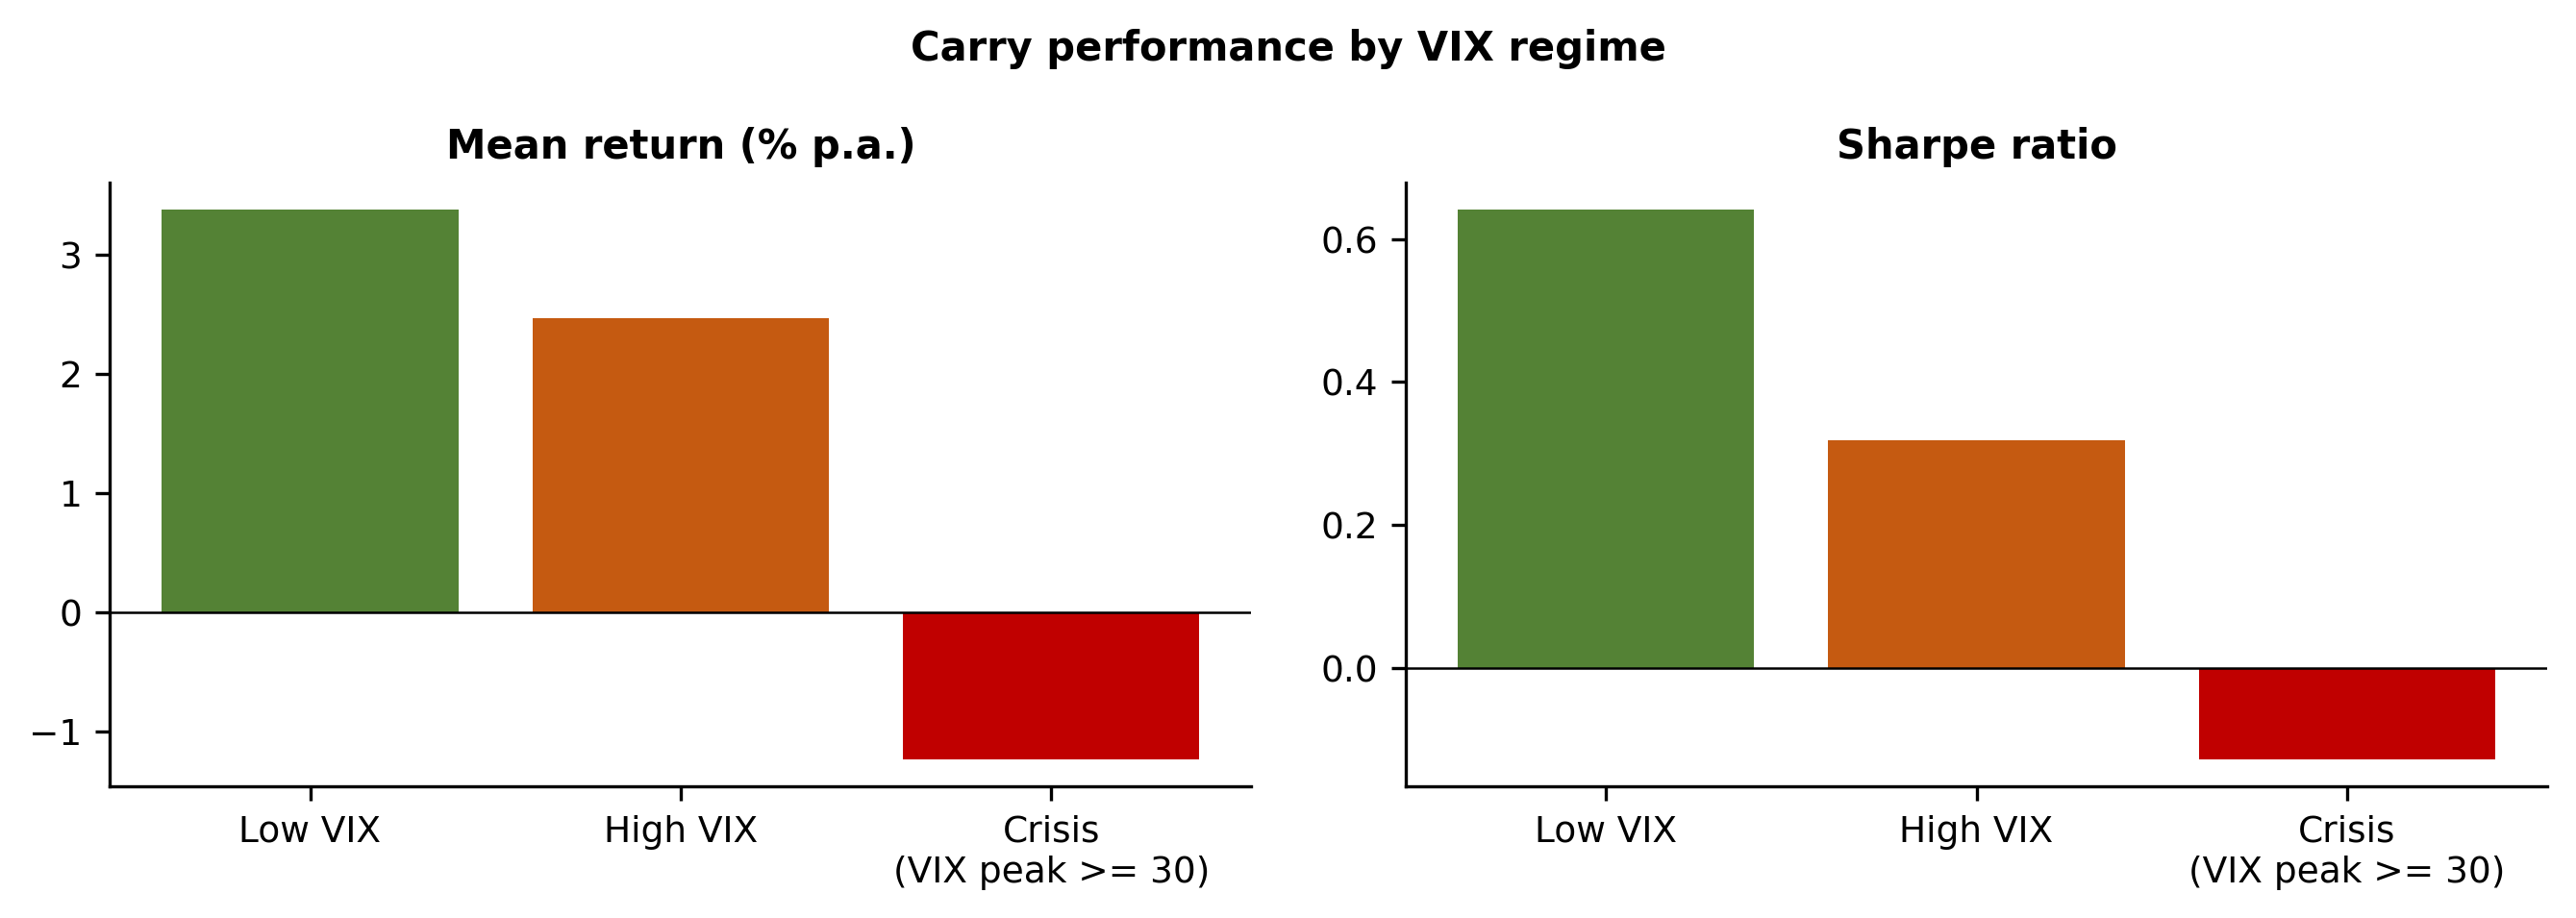
\includegraphics[width=0.7\textwidth]{figures/F08_vix_regimes.png}\caption{Average return and Sharpe ratio of carry in low-VIX, high-VIX and crisis months.}\label{fig:reg}\end{figure}

\section{Results: UIP and the Forward Premium Puzzle}
\begin{table}[H]\centering\small
\caption{UIP test (Fama regression), monthly data, annualised}\label{tab:uip}
\begin{tabularx}{\textwidth}{lCCCCCCC}
\toprule Currency & $\beta$ & Std. error & t ($\beta=0$) & t ($\beta=1$) & p-value ($\beta=1$) & R$^2$ & Months \\ \midrule
EUR & 1.71 & 2.84 & 0.60 & 0.25 & 0.801 & 0.003 & 119 \\
GBP & 0.65 & 3.67 & 0.18 & $-$0.09 & 0.925 & 0.000 & 119 \\
JPY & 1.01 & 1.66 & 0.61 & 0.01 & 0.993 & 0.003 & 119 \\
CHF & 2.45 & 1.76 & 1.39 & 0.82 & 0.412 & 0.014 & 119 \\
NOK & $-$3.01 & 4.17 & $-$0.72 & $-$0.96 & 0.337 & 0.002 & 119 \\
AUD & $-$2.11 & 3.31 & $-$0.64 & $-$0.94 & 0.347 & 0.002 & 119 \\
NZD & 2.55 & 3.40 & 0.75 & 0.46 & 0.648 & 0.002 & 119 \\
CAD & 3.95 & 3.28 & 1.20 & 0.90 & 0.369 & 0.011 & 119 \\
Pooled & 1.15 & 1.61 & 0.71 & 0.09 & 0.926 & 0.004 & 952 \\
\bottomrule\end{tabularx}
\par\vspace{0.3em}\footnotesize\emph{UIP holds if $\beta = 1$; a random walk gives $\beta = 0$. Pooled = all currencies together with currency fixed effects and standard errors clustered by month.}
\end{table}

\textbf{Currency by currency.} Slopes range from $-$3.0 (NOK) to 3.9 (CAD); pooled 1.15 (s.e. 1.61)
(Table~\ref{tab:uip}, Figure~\ref{fig:uip}). No currency rejects UIP, but none rejects a random walk either, and R$^2$ is
below 1.4\%. Ten years of monthly data cannot settle the question: rate gaps moved with the US cycle, while exchange rates
were driven by much larger shocks.

\begin{figure}[!htbp]\centering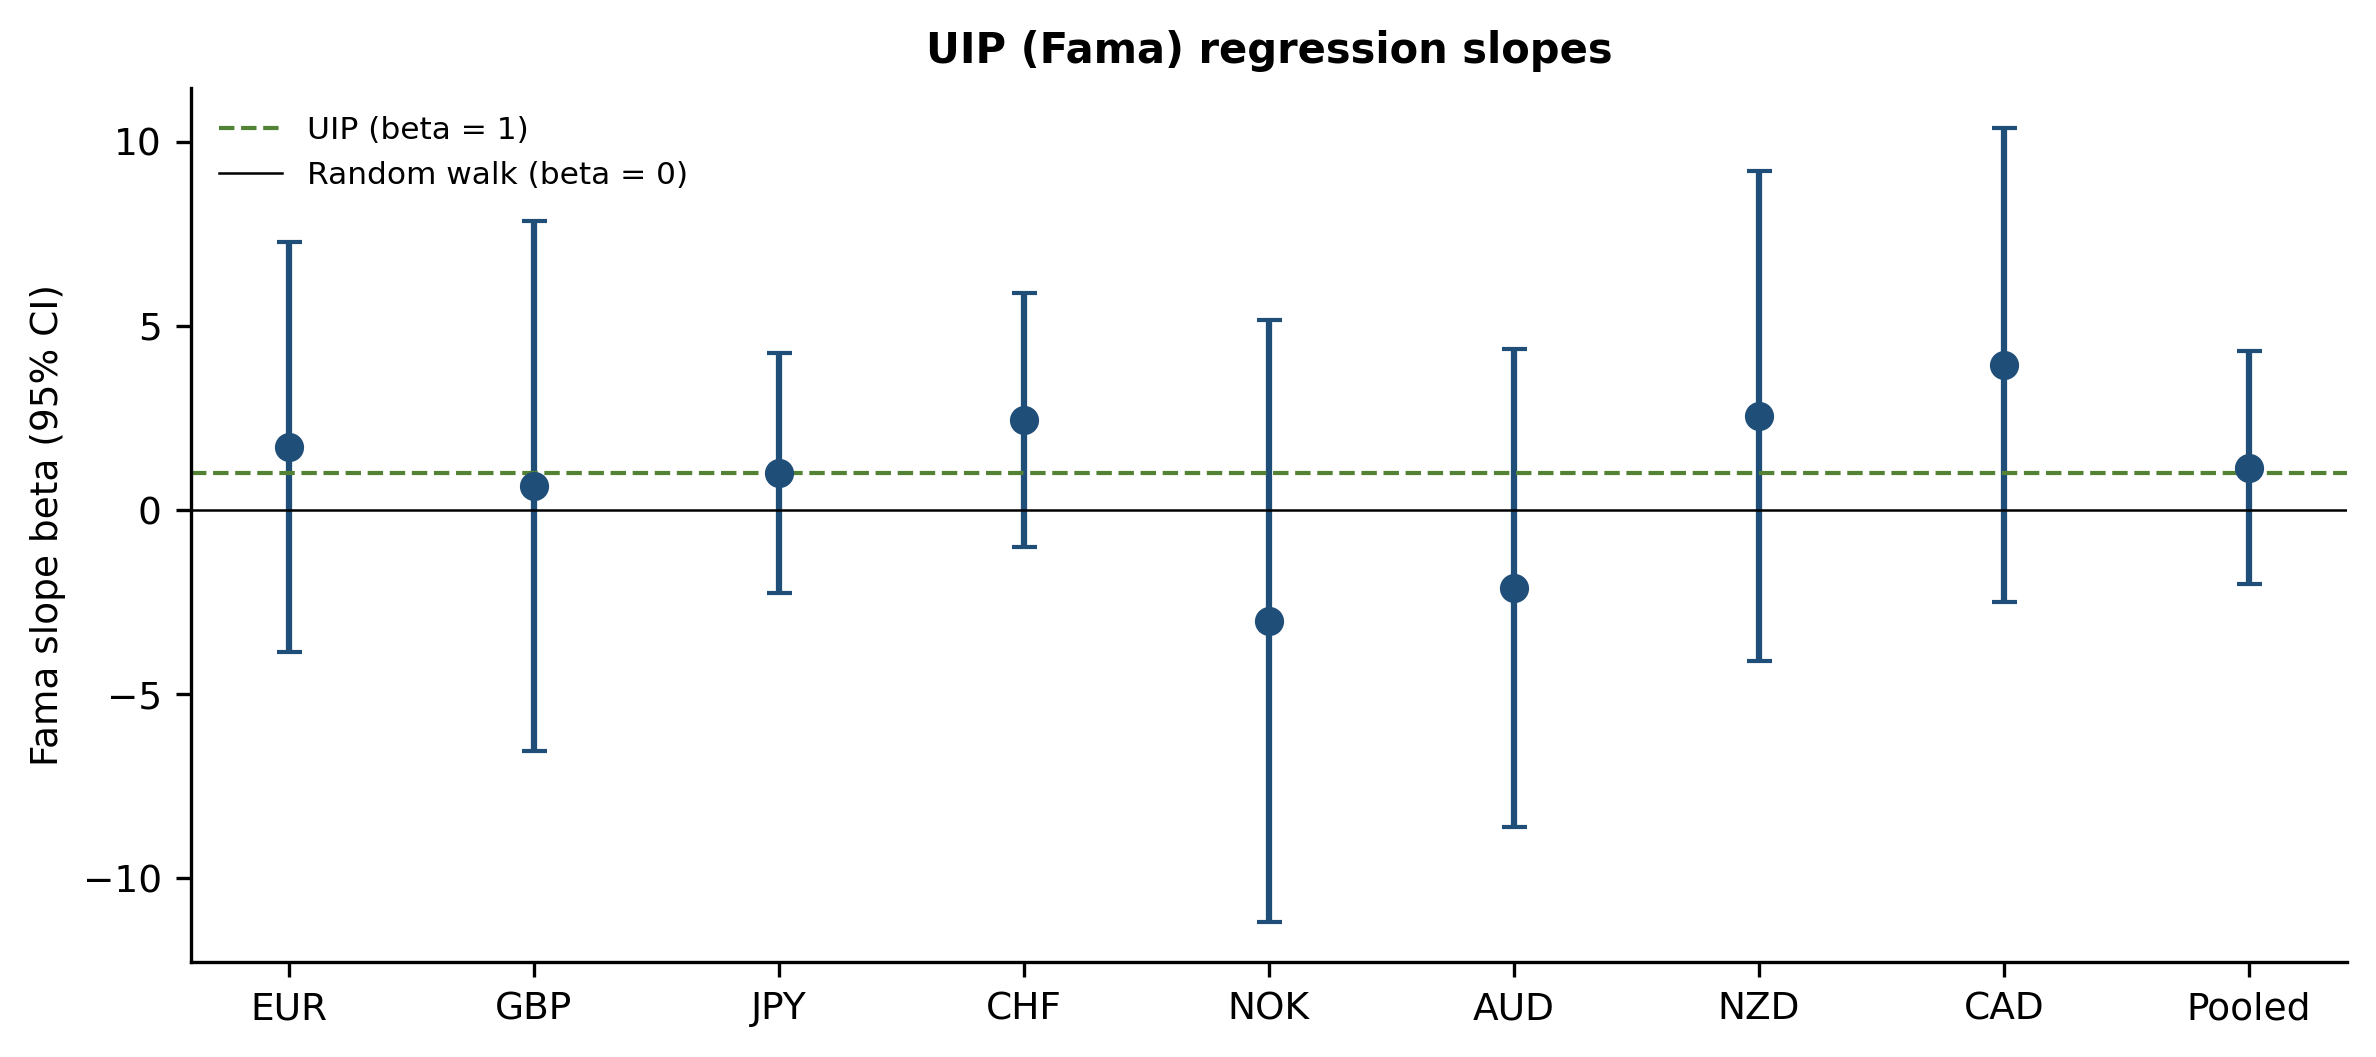
\includegraphics[width=0.7\textwidth]{figures/F09_uip_betas.png}\caption{UIP slopes with 95\% confidence intervals. UIP predicts $\beta = 1$ (dashed line).}\label{fig:uip}\end{figure}

\begin{table}[!htbp]\centering\small
\caption{UIP at the portfolio level (\% per year)}\label{tab:uipp}
\begin{tabularx}{\textwidth}{p{5.5cm}CCC}
\toprule  & Long basket & Short basket & Long minus short \\ \midrule
Average rate gap vs USD (carry) & $-$0.13 & $-$2.60 & +2.48 \\
Actual spot change vs USD & +0.26 & $-$0.23 & +0.49 \\
Spot change UIP predicts & +0.13 & +2.60 & $-$2.48 \\
\bottomrule\end{tabularx}
\end{table}

\textbf{Portfolio level.} The portfolio test is clearer (Table~\ref{tab:uipp}). The sold currencies paid 2.6
points less than USD, so UIP says they should have risen 2.6\% a year; they fell 0.23\%. Long minus short, UIP predicts a
spot loss of 2.48\%; the actual result was a gain of 0.49\%. The yen paid 2.9 points less than the dollar and still fell
3.8\% a year as the Bank of Japan stayed near zero while the Fed went to 5.25--5.50\%. This is the forward premium puzzle.

\textbf{Implication.} The carry return is the rate gap; the risk is in the spot part, which Sections 7 and 8 examine. Ranking
on policy rates instead of forwards gives a similar result (Sharpe 0.35).

\section{Results: Crash Risk}
\textbf{Shape of returns.} Monthly skewness is $-$0.54 and excess kurtosis 0.99; daily figures are $-$0.74 and 8.2. The tail
ratio is 1.08: the six worst months averaged $-$4.36\% against $+$4.02\% for the six best. The dollar basket, by contrast, is
symmetric (skewness 0.03). The pattern matches \citet{bnp2009}, although milder because G10 rate gaps were small.

\begin{figure}[!htbp]\centering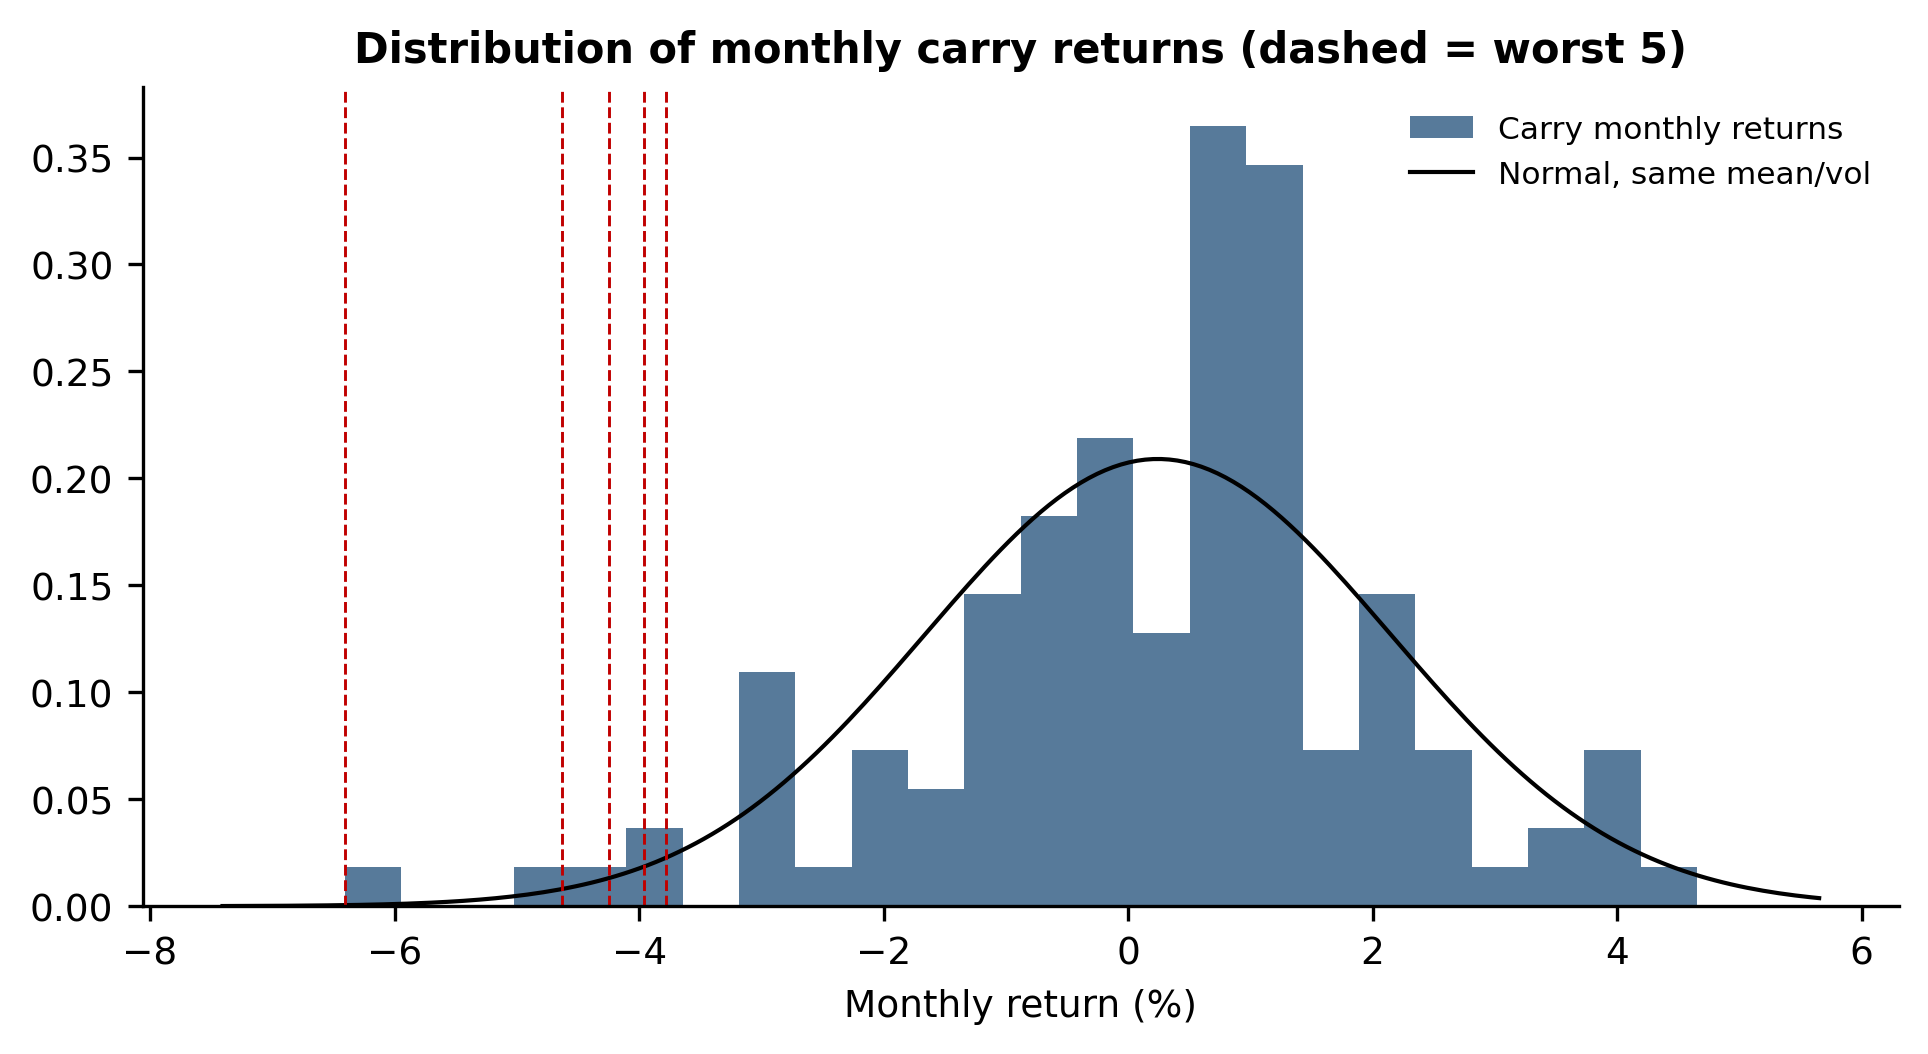
\includegraphics[width=0.55\textwidth]{figures/F06_return_distribution.png}\caption{Monthly carry returns against a normal distribution with the same mean and volatility. Dashed lines mark the five worst months.}\label{fig:dist}\end{figure}

\begin{table}[!htbp]\centering\footnotesize
\caption{The five worst months and what caused them}\label{tab:worst}
\begin{tabularx}{\textwidth}{p{1.1cm}p{1.0cm}p{1.0cm}p{1.0cm}>{\raggedright\arraybackslash}p{2.3cm}p{0.6cm}Y}
\toprule Month & Return (\%) & Long side (\%) & Short side (\%) & Long / short & VIX & What happened \\ \midrule
2020-03 & $-$6.41 & $-$6.35 & $-$0.06 & NOK, NZD, CAD / EUR, JPY, CHF & 57.7 & COVID-19 declared a pandemic; Saudi--Russia oil price war (9 Mar) hit NOK and CAD; rush into dollars; Fed cut rates to zero (15 Mar). \\
2018-12 & $-$4.63 & $-$2.82 & $-$1.81 & AUD, NZD, CAD / EUR, JPY, CHF & 24.9 & Fed hiked to 2.25--2.50\% and kept shrinking its balance sheet (19 Dec); oil and stocks fell; US government shutdown (22 Dec). \\
2021-11 & $-$4.25 & $-$4.81 & 0.56 & NOK, NZD, CAD / EUR, JPY, CHF & 18.5 & Omicron variant (26 Nov) caused an oil sell-off that hit NOK and CAD; Fed dropped the word ``transitory'' (30 Nov). \\
2022-09 & $-$3.96 & $-$6.67 & 2.71 & AUD, NZD, CAD / EUR, JPY, CHF & 27.3 & Fed hiked 75 bp (21 Sep) and the dollar peaked; UK mini-budget crisis (23 Sep); Japan bought yen for the first time since 1998 (22 Sep). \\
2024-07 & $-$3.78 & $-$0.56 & $-$3.22 & GBP, NZD, CAD / EUR, JPY, CHF & 14.4 & Japan intervened to support the yen (11--12 Jul) and the BoJ hiked (31 Jul); the yen jumped and the short-yen leg lost; the unwind peaked on 5 Aug. \\
\bottomrule\end{tabularx}
\par\vspace{0.3em}\footnotesize\emph{Long/short basket = contribution of each side to the monthly return.}
\end{table}

\textbf{Linking crashes to events.} All five worst months were global sell-offs (Table~\ref{tab:worst},
Figure~\ref{fig:contrib}), and all losses came from exchange rates, not carry. Two patterns:
\begin{itemize}\setlength{\itemsep}{0pt}
\item \textbf{Long basket fell} (Mar 2020, Dec 2018, Nov 2021, Sep 2022): NOK, NZD, AUD and CAD fell with oil and equities as
the dollar rose.
\item \textbf{Short basket rose} (Jul 2024): the yen jumped on the BoJ hike and Japanese intervention, forcing yen-funded
traders to unwind at once --- the 2008 pattern again.
\end{itemize}

\begin{figure}[!htbp]\centering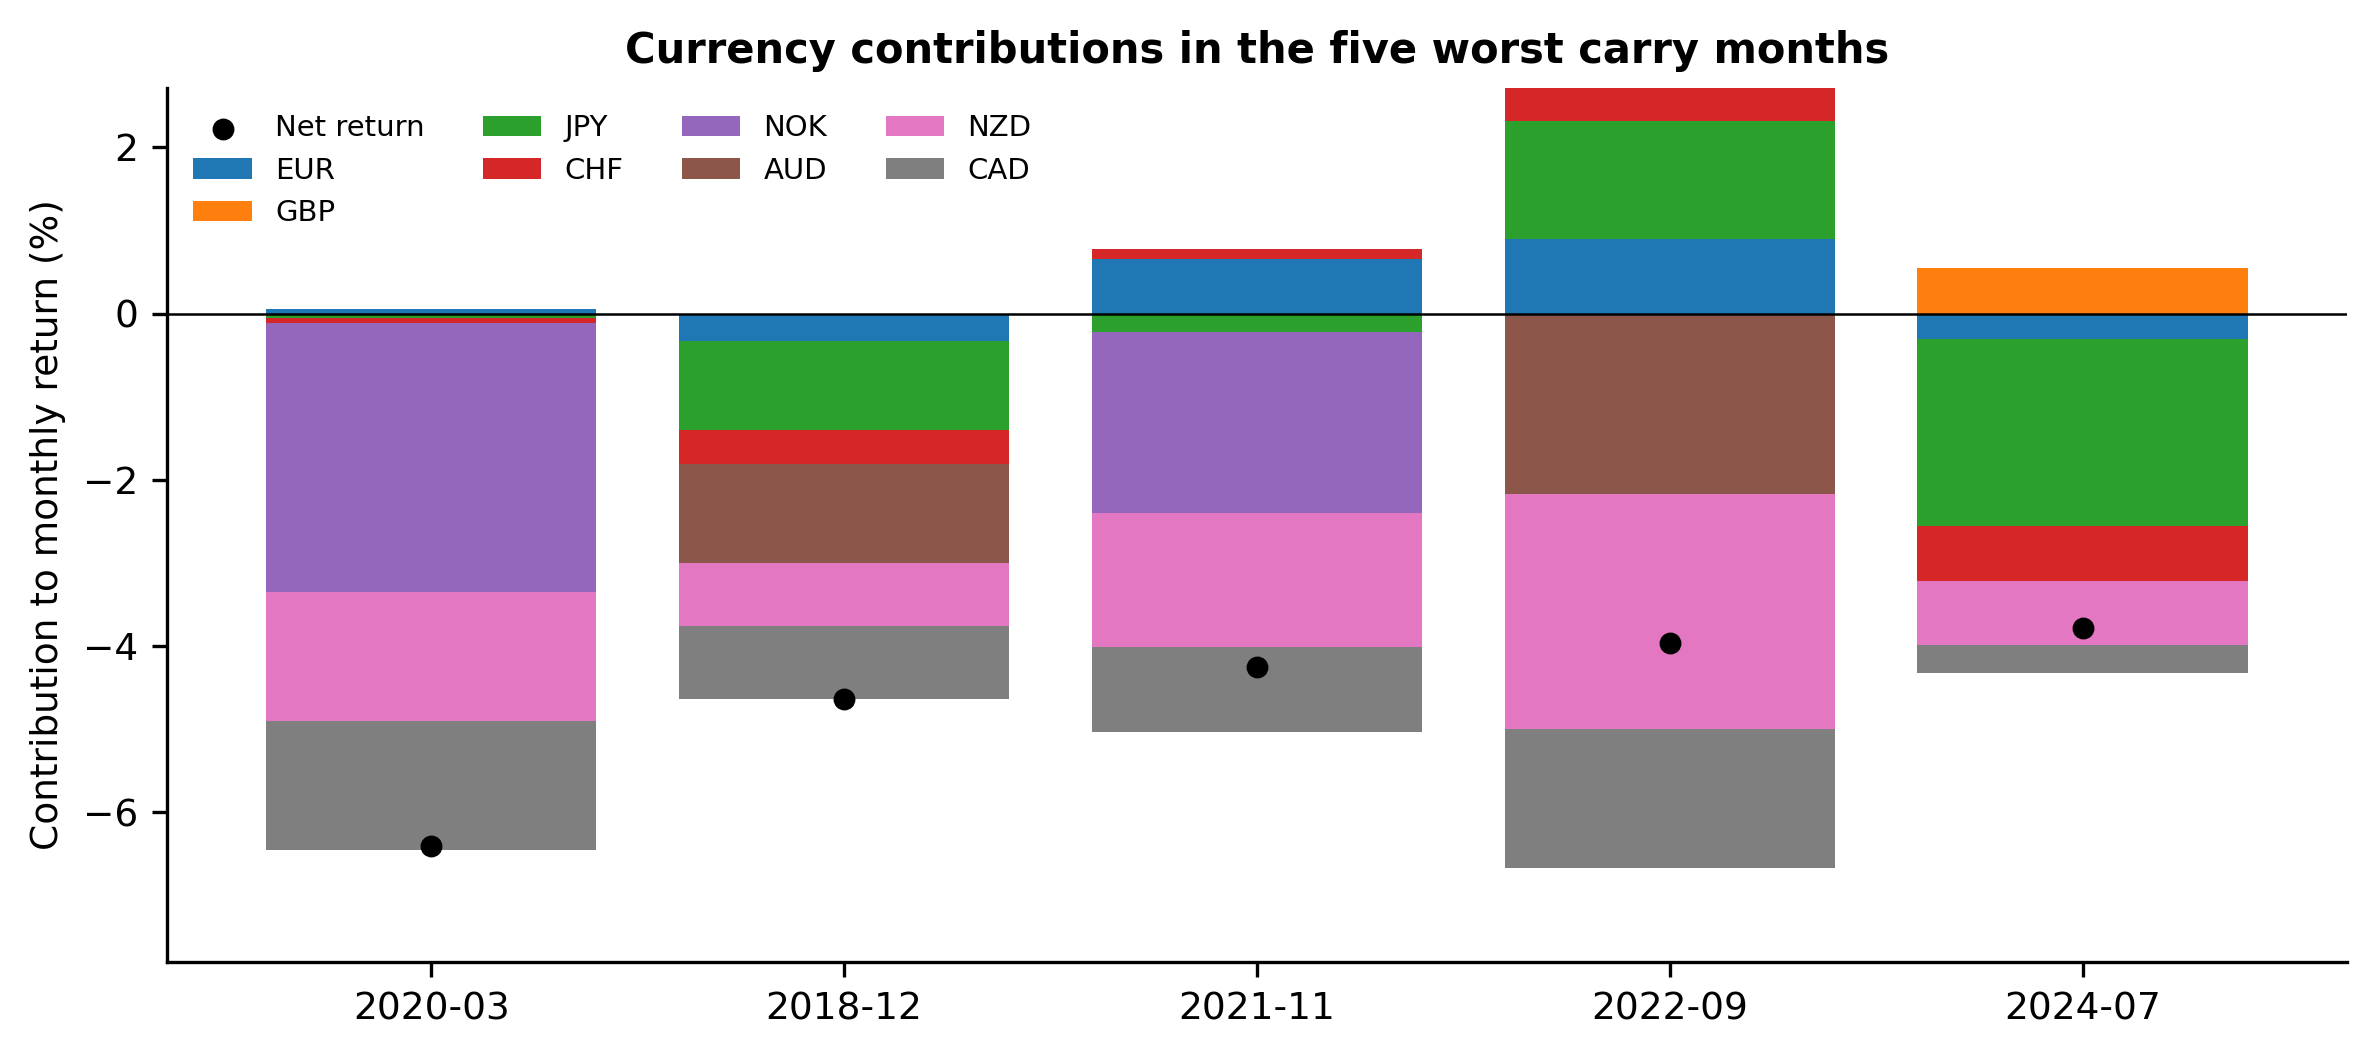
\includegraphics[width=0.72\textwidth]{figures/F11_worst_month_contributions.png}\caption{Contribution of each currency to the return in the five worst months (dots = total).}\label{fig:contrib}\end{figure}

Seven of the ten worst days were in March 2020 or April 2025 (Annex Table~\ref{tab:days}). In April
2025 the dollar fell, yet carry lost 3.0\% because CHF, JPY and EUR rose even faster than the high-rate currencies: carry
crash risk is about safe havens versus risky currencies, not the dollar. The 2026 Iran-war oil shock did not hurt
(March 2026: $+$0.6\%), since the strategy was long NOK and AUD and short oil importers JPY and EUR.

\section{Results: Is Carry a Risk Factor?}
\begin{table}[!htbp]\centering\small
\caption{Correlation of carry with the S\&P 500 and the VIX}\label{tab:corr}
\begin{tabularx}{\textwidth}{lCCCC}
\toprule Period & Monthly: S\&P 500 & Monthly: VIX change & Daily: S\&P 500 & Daily: VIX change \\ \midrule
Full sample & 0.56 & $-$0.57 & 0.58 & $-$0.52 \\
2016-09 to 2019-12 & 0.53 & $-$0.61 & 0.53 & $-$0.43 \\
2020-01 to 2022-12 & 0.72 & $-$0.66 & 0.64 & $-$0.56 \\
2023-01 to end & 0.20 & $-$0.31 & 0.52 & $-$0.53 \\
\bottomrule\end{tabularx}
\end{table}

\textbf{Correlation over time.} Carry moves with equities: correlation 0.56 with the S\&P 500 and $-$0.57 with
VIX changes (monthly; Table~\ref{tab:corr}). The rolling one-year correlation (Figure~\ref{fig:roll}) stayed between 0.30 and
0.79: about 0.75 after March 2020, 0.30--0.40 in calm 2023--24, and back near 0.7 after April 2025. It rises exactly when
diversification is needed --- the mark of a risk factor.

\begin{figure}[!htbp]\centering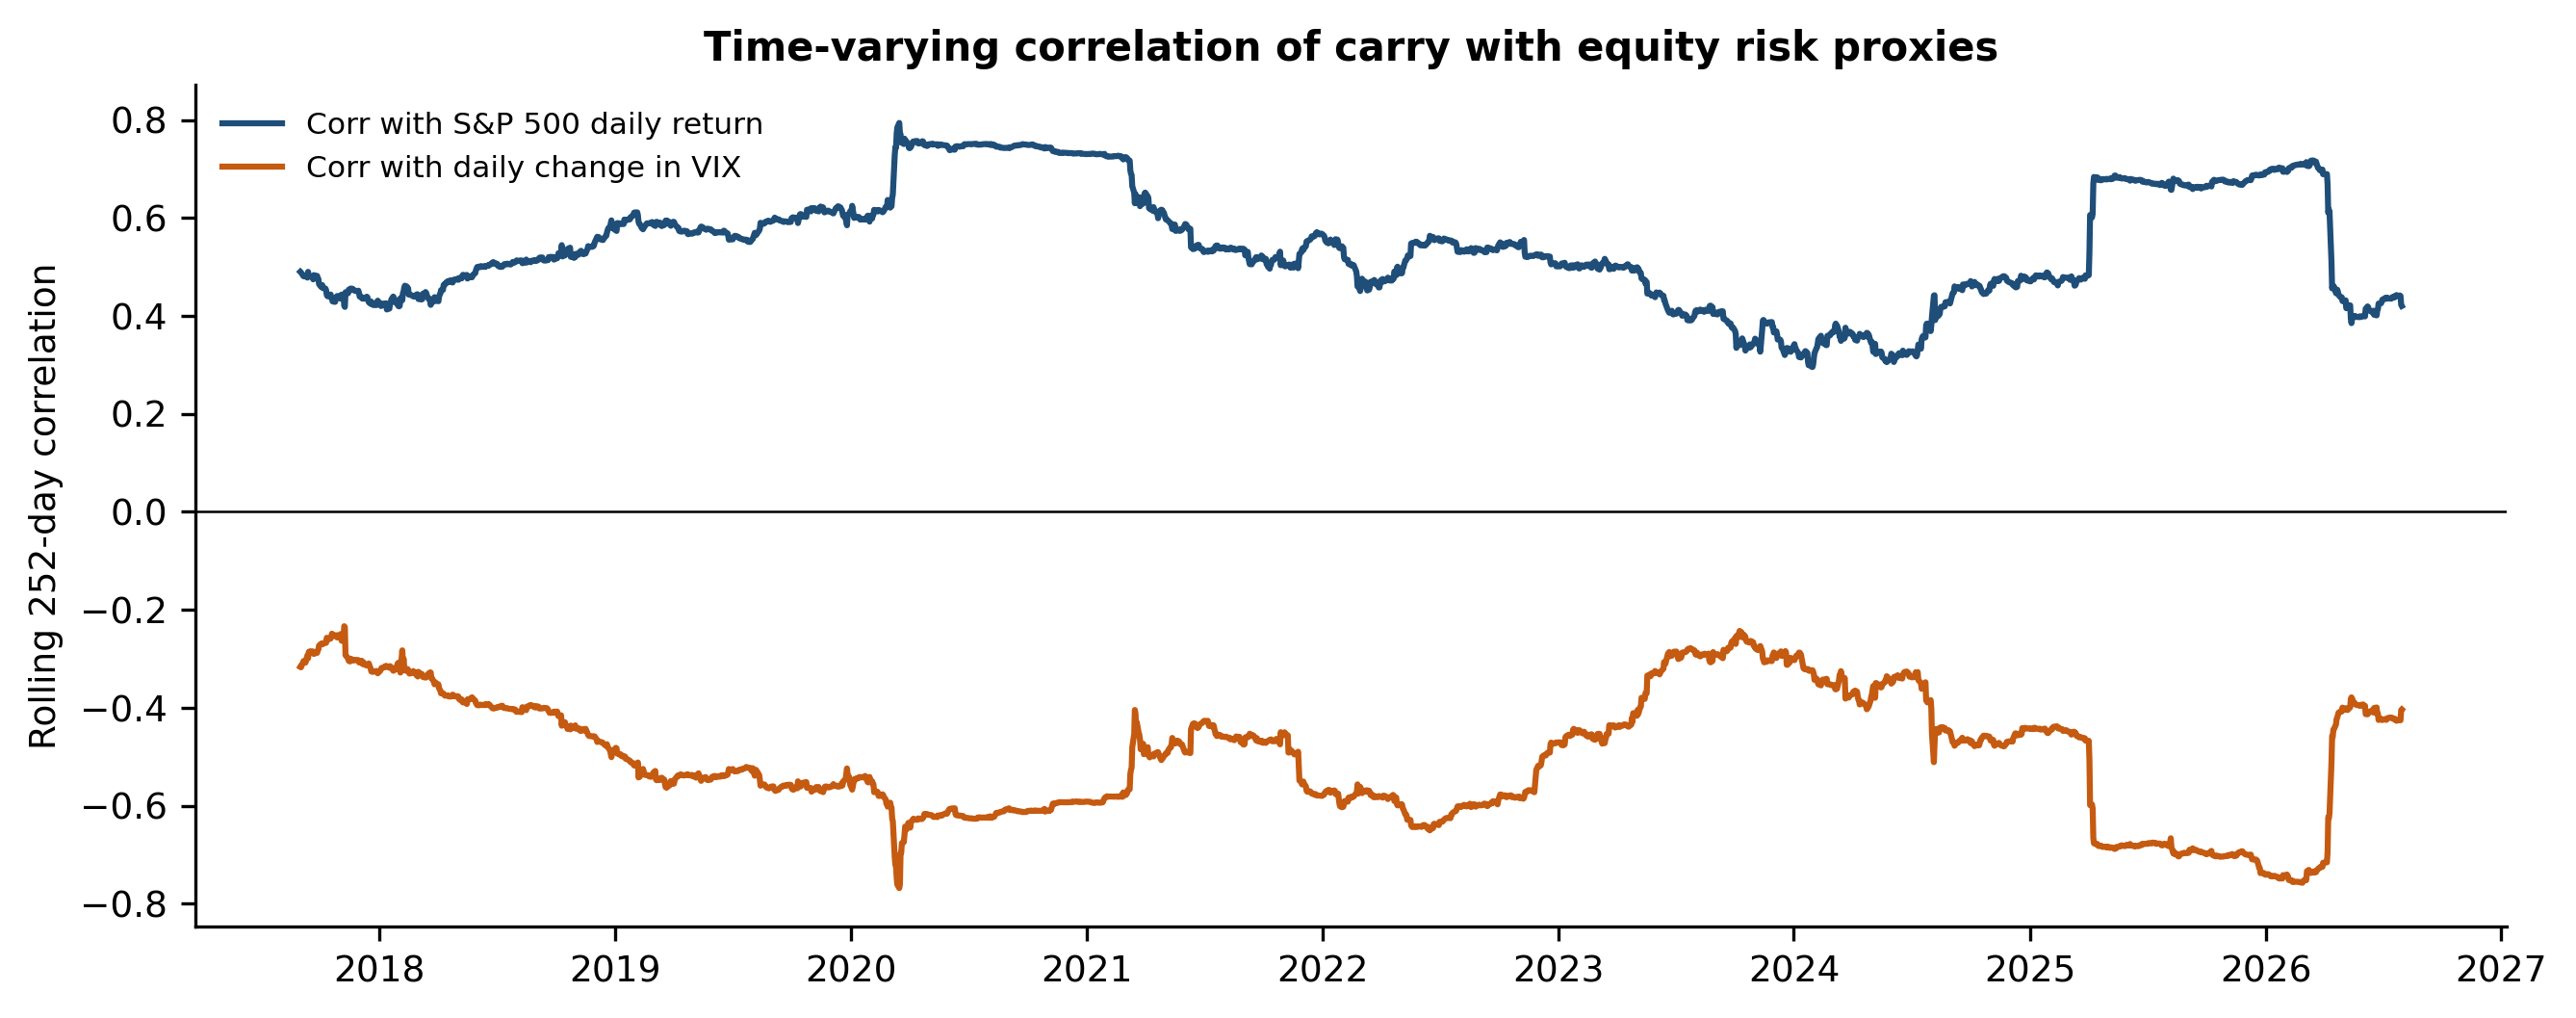
\includegraphics[width=0.8\textwidth]{figures/F07_rolling_correlations.png}\caption{Rolling one-year (252-day) correlation of daily carry returns with the S\&P 500 and with daily VIX changes.}\label{fig:roll}\end{figure}

\begin{table}[!htbp]\centering\small
\caption{Carry regressed on market risk (dependent variable: monthly carry return, \%)}\label{tab:risk}
\begin{tabularx}{\textwidth}{p{4.5cm}CCCCC}
\toprule Risk measure & $\alpha$ (\% per month) & t($\alpha$) & $\beta$ & t($\beta$) & R$^2$ \\ \midrule
S\&P 500 return & $-$0.032 & $-$0.22 & 0.240 & 6.24 & 0.31 \\
Change in VIX & 0.247 & 2.13 & $-$0.199 & $-$8.76 & 0.33 \\
Global FX volatility shock & 0.248 & 1.87 & $-$4.910 & $-$2.03 & 0.07 \\
S\&P 500 and VIX change together & 0.105 & 0.73 & 0.123 & 2.19 & 0.36 \\
\bottomrule\end{tabularx}
\par\vspace{0.3em}\footnotesize\emph{$\beta$ on the S\&P 500: carry return per 1\% S\&P move. $\beta$ on the VIX: carry return (\%) per VIX point. FX volatility shock = unexpected change in average daily moves of the eight currencies.}
\end{table}

\textbf{Risk-adjusted return.} The S\&P 500 alone explains 31\% of carry's variation ($\beta$ = 0.24) and VIX
changes 33\% ($-$0.20\% per VIX point); FX volatility shocks also hurt (Table~\ref{tab:risk}). With both controls, the alpha
falls from 0.24\% to 0.10\% a month and is insignificant (t = 0.73).

\begin{table}[!htbp]\centering\small
\caption{Fama--MacBeth test: is carry risk priced? (\% per month)}\label{tab:fmb}
\begin{tabularx}{\textwidth}{p{6cm}CC}
\toprule  & Estimate & t-statistic \\ \midrule
Constant & 0.123 & 0.60 \\
Price of dollar risk & $-$0.263 & $-$1.06 \\
Price of carry risk & 0.233 & 1.49 \\
Average return of DOL & $-$0.141 & $-$0.82 \\
Average return of carry factor & 0.247 & 1.83 \\
R$^2$ across currencies & 0.461 & -- \\
\bottomrule\end{tabularx}
\par\vspace{0.3em}\footnotesize\emph{If the factor is priced correctly, its price of risk should equal its average return. 8 currencies, 119 months.}
\end{table}

\textbf{Priced like a Fama--French factor?} Funding currencies have negative carry betas (JPY $-$0.82, CHF
$-$0.51, EUR $-$0.32) and high-rate currencies positive ones (AUD 0.48, NOK 0.45, NZD 0.42, CAD 0.31; Annex
Table~\ref{tab:betas}). The estimated price of carry risk (0.233\% a month) is almost equal to the factor's average return
(0.247\%), and the two factors explain 46\% of cross-currency returns (Table~\ref{tab:fmb}). With eight currencies the
estimate is imprecise (t = 1.49), so this supports, but does not prove, a priced carry factor.

\section{Results: Momentum Filter}
\begin{table}[!htbp]\centering\small
\caption{Carry with and without the three-month momentum filter (December 2016 -- July 2026, 116 months, net)}\label{tab:mom}
\begin{tabularx}{\textwidth}{p{4.2cm}CCCCCC}
\toprule Strategy & Return (\% p.a.) & Volatility (\% p.a.) & Sharpe & Max drawdown (\%) & Skewness & t-stat \\ \midrule
Carry & 2.52 & 6.64 & 0.38 & $-$14.04 & $-$0.51 & 1.55 \\
Carry + momentum filter & $-$1.63 & 7.25 & $-$0.23 & $-$29.00 & $-$0.05 & $-$0.73 \\
Carry and momentum combined rank & $-$1.80 & 5.16 & $-$0.35 & $-$28.07 & $-$0.54 & $-$1.09 \\
Momentum only (reference) & $-$5.41 & 5.83 & $-$0.93 & $-$44.88 & 0.43 & $-$2.84 \\
\bottomrule\end{tabularx}
\par\vspace{0.3em}\footnotesize\emph{Filter: keep a long only if the currency rose over the last three months, and a short only if it fell. Combined rank: average of the carry rank and the momentum rank. Momentum only: buy the three best and sell the three worst performers of the last three months.}
\end{table}

The filter made things worse (Table~\ref{tab:mom}): $-$1.63\% a year (Sharpe $-$0.23) against $+$2.52\%
(Sharpe 0.38) for plain carry, with twice the drawdown. Pure three-month momentum lost 5.41\% a year (t = $-$2.84): major
currencies reversed at this horizon, so the filter dropped positions just before they recovered, in line with
\citet{msss2012b}. It also left one side empty in a quarter to a third of months (a hidden dollar bet) and raised turnover
from 8\% to 62\%. It helped slightly in crises (Sharpe 0.04 vs $-$0.13) but cost far more in calm markets ($-$0.70 vs 0.64).
Volatility-based sizing or option hedges \citep{jurek2014} are better crash protection.

\section{Discussion}
\textbf{Risk premium or inefficiency?} A risk premium: the return is the rate gap, earned slowly and lost in global
sell-offs; returns are left-skewed; carry moves with equities and against the VIX, more so in crises; alpha disappears after
risk controls; and the price of carry risk matches its mean. Two cautions: significance is only at 10\%, and the result rests
on one trade --- short CHF, JPY and EUR against a high-yielding dollar. The long basket alone made only 0.13\% a year.

\textbf{Costs and robustness.} Raising costs from 0 to 20 bp only lowers the Sharpe from 0.45 to 0.42 (Annex
Table~\ref{tab:rob}); FXIP forward spreads (e.g. 15.03/15.09 for EURUSD) imply under 1 bp a month. Policy-rate ranking
(Sharpe 0.35) and two-by-two legs (0.40) give similar results.

\textbf{Capacity.} USD, EUR and JPY are the most traded currencies \citep{bis2025}, so size is not the limit; crowding is.
When many leveraged traders fund in the same currency, as with the yen in 2007 and 2024, the unwind becomes the crash.

\textbf{Outlook (WIRP).} On 17 August 2026 WIRP ranks the currencies like the forwards do (rank correlation 0.98; Annex
Table~\ref{tab:wirp}). The current portfolio is long AUD, NOK, GBP and short CHF, JPY, CAD. Markets price about 82 bp of
BoJ hikes against 38 bp from the Fed, so the yen funding gap is expected to shrink --- the set-up behind the 2024 crash.

\textbf{Limitations.} Eight currencies; one deep crisis in the sample; daily returns approximated; fixed costs; WIRP is one
snapshot and positioning data were unavailable.

\section{Conclusion}
A simple G10 carry strategy made 2.9\% a year (Sharpe 0.44) in 2016--2026, beating static carry and a dollar basket. It was
short CHF, JPY and EUR almost every month and rotated its longs among AUD, NZD, CAD, NOK and GBP. The return was the rate
gap: low-rate currencies, especially the yen, did not rise as UIP predicts. The cost is crash risk --- left-skewed returns,
losses in global shocks and crises, and higher equity correlation under stress. Equity and volatility risk explain most of
the return, so carry is a risk premium, not a market error. Momentum filters do not help; sizing and option hedges are
better tools. With the BoJ now hiking, the short-yen trade that drove the decade's profits is also its biggest risk.

\begin{thebibliography}{99}\setlength{\itemsep}{2pt}\small
\bibitem[Bank for International Settlements(2024)]{bis2024} Bank for International Settlements. (2024, September). \emph{BIS Quarterly Review: International banking and financial market developments}. BIS. https://www.bis.org/publ/qtrpdf/r\_qt2409.htm
\bibitem[Bank for International Settlements(2025)]{bis2025} Bank for International Settlements. (2025). \emph{Triennial Central Bank Survey of foreign exchange and over-the-counter (OTC) derivatives markets in 2025}. BIS. https://www.bis.org/statistics/rpfx25.htm
\bibitem[Brunnermeier et~al.(2009)]{bnp2009} Brunnermeier, M. K., Nagel, S., \& Pedersen, L. H. (2009). Carry trades and currency crashes. \emph{NBER Macroeconomics Annual, 23}(1), 313--348.
\bibitem[Burnside(2012)]{burnside2012} Burnside, C. (2012). Carry trades and risk. In J. James, I. Marsh, \& L. Sarno (Eds.), \emph{Handbook of exchange rates} (pp. 283--312). Wiley.
\bibitem[Burnside et~al.(2011)]{burnside2011} Burnside, C., Eichenbaum, M., Kleshchelski, I., \& Rebelo, S. (2011). Do peso problems explain the returns to the carry trade? \emph{Review of Financial Studies, 24}(3), 853--891.
\bibitem[Daniel et~al.(2017)]{dhl2017} Daniel, K., Hodrick, R. J., \& Lu, Z. (2017). The carry trade: Risks and drawdowns. \emph{Critical Finance Review, 6}(2), 211--262.
\bibitem[Du et~al.(2018)]{dtv2018} Du, W., Tepper, A., \& Verdelhan, A. (2018). Deviations from covered interest rate parity. \emph{Journal of Finance, 73}(3), 915--957.
\bibitem[Engel(1996)]{engel1996} Engel, C. (1996). The forward discount anomaly and the risk premium: A survey of recent evidence. \emph{Journal of Empirical Finance, 3}(2), 123--192.
\bibitem[Fama(1984)]{fama1984} Fama, E. F. (1984). Forward and spot exchange rates. \emph{Journal of Monetary Economics, 14}(3), 319--338.
\bibitem[Fama and MacBeth(1973)]{fm1973} Fama, E. F., \& MacBeth, J. D. (1973). Risk, return, and equilibrium: Empirical tests. \emph{Journal of Political Economy, 81}(3), 607--636.
\bibitem[Hansen and Hodrick(1980)]{hansenhodrick1980} Hansen, L. P., \& Hodrick, R. J. (1980). Forward exchange rates as optimal predictors of future spot rates: An econometric analysis. \emph{Journal of Political Economy, 88}(5), 829--853.
\bibitem[Jurek(2014)]{jurek2014} Jurek, J. W. (2014). Crash-neutral currency carry trades. \emph{Journal of Financial Economics, 113}(3), 325--347.
\bibitem[Koijen et~al.(2018)]{koijen2018} Koijen, R. S. J., Moskowitz, T. J., Pedersen, L. H., \& Vrugt, E. B. (2018). Carry. \emph{Journal of Financial Economics, 127}(2), 197--225.
\bibitem[Lustig et~al.(2011)]{lrv2011} Lustig, H., Roussanov, N., \& Verdelhan, A. (2011). Common risk factors in currency markets. \emph{Review of Financial Studies, 24}(11), 3731--3777.
\bibitem[Menkhoff et~al.(2012a)]{msss2012a} Menkhoff, L., Sarno, L., Schmeling, M., \& Schrimpf, A. (2012a). Carry trades and global foreign exchange volatility. \emph{Journal of Finance, 67}(2), 681--718.
\bibitem[Menkhoff et~al.(2012b)]{msss2012b} Menkhoff, L., Sarno, L., Schmeling, M., \& Schrimpf, A. (2012b). Currency momentum strategies. \emph{Journal of Financial Economics, 106}(3), 660--684.
\bibitem[Newey and West(1987)]{nw1987} Newey, W. K., \& West, K. D. (1987). A simple, positive semi-definite, heteroskedasticity and autocorrelation consistent covariance matrix. \emph{Econometrica, 55}(3), 703--708.
\end{thebibliography}
\noindent{\small Data: Bloomberg L.P. (2026), GP, FRD, WIRP and FXIP functions, accessed August 2026. Event dates: official releases of
the Federal Reserve, ECB, Bank of Japan, Bank of England, Swiss National Bank, Norges Bank, RBA, RBNZ, Bank of Canada and
Japan's Ministry of Finance.}

\clearpage
\appendix
\section*{Annexures}
\addcontentsline{toc}{section}{Annexures}
\setcounter{table}{0}\renewcommand{\thetable}{A\arabic{table}}
\setcounter{figure}{0}\renewcommand{\thefigure}{A\arabic{figure}}
\subsection*{Annex A. Additional results}

\begin{table}[!htbp]\centering\small
\caption{Yearly returns (\%)}\label{tab:annual}
\begin{tabularx}{\textwidth}{lCCCCC}
\toprule Year & Carry (net) & Carry + momentum & Static carry & Dollar basket & Months \\ \midrule
2016 & +3.89 & +1.18 & +3.89 & $-$5.33 & 4 \\
2017 & +1.61 & $-$11.02 & +0.40 & +6.05 & 12 \\
2018 & $-$4.57 & $-$11.40 & $-$3.72 & $-$5.93 & 12 \\
2019 & +2.80 & $-$3.38 & +1.40 & $-$0.81 & 12 \\
2020 & $-$0.71 & $-$2.93 & $-$0.16 & +5.41 & 12 \\
2021 & +4.60 & $-$1.89 & +3.14 & $-$4.49 & 12 \\
2022 & +0.50 & +1.16 & +0.61 & $-$8.29 & 12 \\
2023 & +4.09 & +5.82 & $-$0.15 & $-$0.78 & 12 \\
2024 & +4.32 & $-$2.10 & +0.29 & $-$9.64 & 12 \\
2025 & +3.43 & +4.63 & +1.54 & +6.13 & 12 \\
2026 & +7.60 & +3.44 & +7.92 & +0.13 & 7 \\
\bottomrule\end{tabularx}
\par\vspace{0.3em}\footnotesize\emph{2016 covers September--December; 2026 covers January--July.}
\end{table}

\begin{table}[!htbp]\centering\small
\caption{The ten worst days}\label{tab:days}
\begin{tabularx}{\textwidth}{lcccY}
\toprule Date & Carry (\%) & S\&P 500 (\%) & VIX change & Event \\ \midrule
2020-03-09 & $-$3.78 & $-$7.60 & 12.5 & Saudi--Russia oil price war; global stock crash \\
2020-03-18 & $-$3.57 & $-$5.18 & 0.5 & Rush into US dollars \\
2025-04-04 & $-$2.86 & $-$5.97 & 15.3 & China retaliates against US tariffs \\
2020-03-12 & $-$2.38 & $-$9.51 & 21.6 & Stock market crash; ECB disappoints \\
2021-11-26 & $-$2.31 & $-$2.27 & 10.0 & Omicron variant; oil falls 13\% \\
2025-04-10 & $-$2.17 & $-$3.46 & 7.1 & US--China tariff escalation \\
2020-03-16 & $-$2.15 & $-$11.98 & 24.9 & Fed cuts to zero, markets still fall \\
2020-06-11 & $-$1.59 & $-$5.89 & 13.2 & Fed outlook and second-wave fears \\
2022-05-18 & $-$1.57 & $-$4.04 & 4.9 & US retail earnings shock \\
2025-04-03 & $-$1.54 & $-$4.84 & 8.5 & Day after US ``Liberation Day'' tariffs \\
\bottomrule\end{tabularx}
\end{table}

\begin{figure}[!htbp]\centering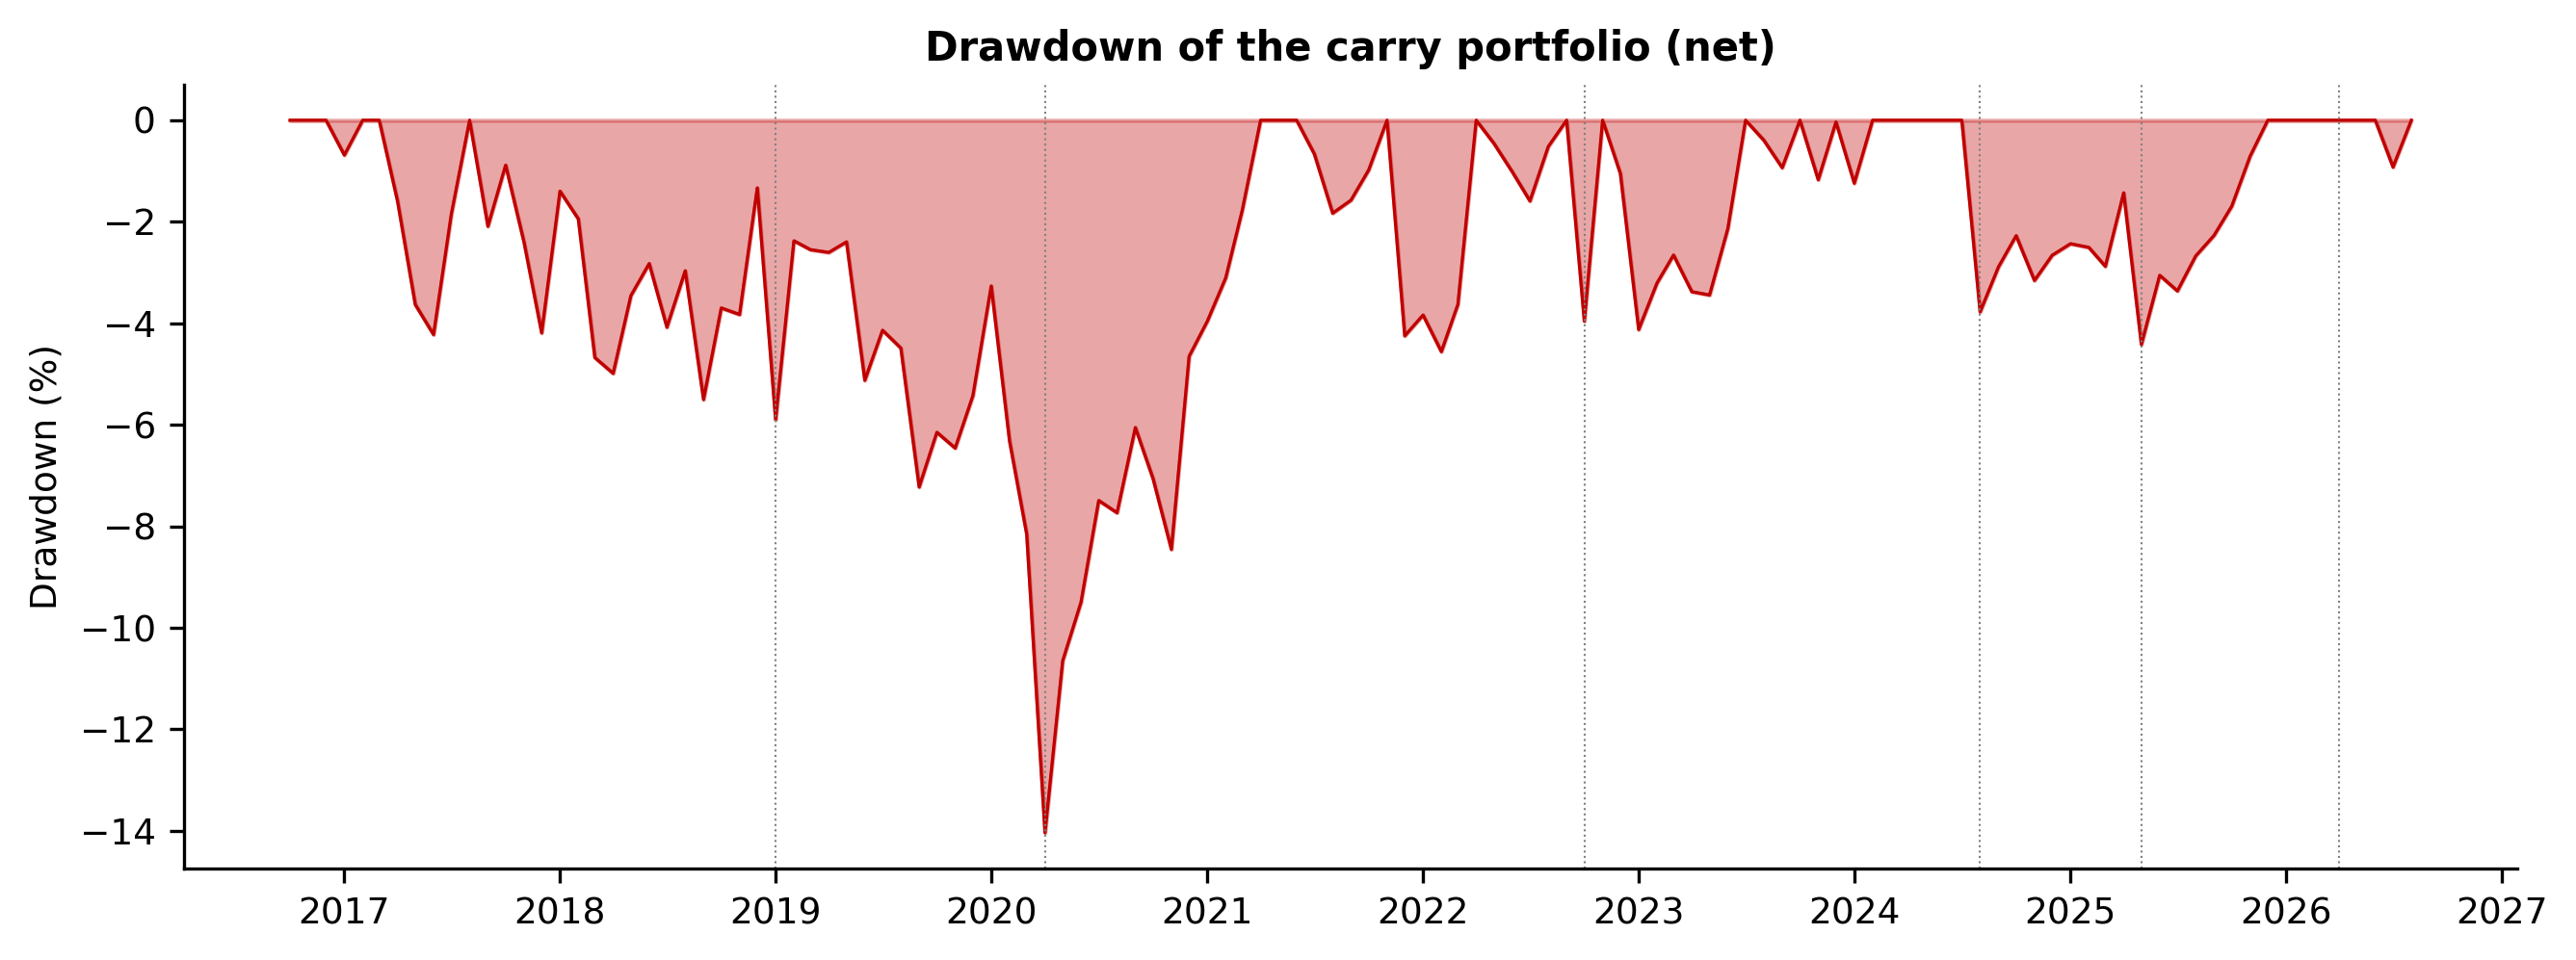
\includegraphics[width=0.75\textwidth]{figures/F05_drawdown.png}\caption{Drawdown of the carry portfolio (net), with the main market shocks marked.}\label{fig:dd}\end{figure}

\begin{table}[!htbp]\centering\small
\caption{Factor betas of each currency (dollar factor and carry factor)}\label{tab:betas}
\begin{tabularx}{\textwidth}{lCCC}
\toprule Currency & Beta to dollar factor & Beta to carry factor & Average return (\% per month) \\ \midrule
EUR & 0.92 & $-$0.32 & $-$0.113 \\
GBP & 0.88 & $-$0.01 & $-$0.009 \\
JPY & 1.04 & $-$0.82 & $-$0.556 \\
CHF & 0.97 & $-$0.51 & $-$0.063 \\
NOK & 1.28 & 0.45 & $-$0.100 \\
AUD & 1.05 & 0.48 & $-$0.052 \\
NZD & 1.22 & 0.42 & $-$0.139 \\
CAD & 0.65 & 0.31 & $-$0.092 \\
\bottomrule\end{tabularx}
\end{table}

\begin{table}[!htbp]\centering\small
\caption{Robustness checks (net)}\label{tab:rob}
\begin{tabularx}{\textwidth}{p{5.5cm}CCC}
\toprule Version & Return (\% p.a.) & Sharpe & Max drawdown (\%) \\ \midrule
0 bps & 2.97 & 0.449 & $-$14.03 \\
2.5 bps & 2.94 & 0.445 & $-$14.03 \\
5 bps & 2.92 & 0.441 & $-$14.04 \\
10 bps & 2.87 & 0.434 & $-$14.05 \\
20 bps & 2.77 & 0.419 & $-$14.08 \\
Forward-discount signal (baseline) & 2.92 & 0.441 & $-$14.04 \\
Policy-rate differential signal & 2.25 & 0.348 & $-$15.44 \\
Top-2 / bottom-2 (forward signal) & 2.91 & 0.395 & $-$14.49 \\
\bottomrule\end{tabularx}
\end{table}

\begin{table}[!htbp]\centering\small
\caption{Five largest drawdowns (net, monthly)}\label{tab:dd}
\begin{tabularx}{\textwidth}{CCCC}
\toprule Start & Lowest point & Recovered & Depth (\%) \\ \midrule
2017-08 & 2020-03 & 2021-03 & $-$14.04 \\
2021-11 & 2022-01 & 2022-03 & $-$4.56 \\
2024-07 & 2025-04 & 2025-11 & $-$4.42 \\
2017-03 & 2017-05 & 2017-07 & $-$4.22 \\
2022-11 & 2022-12 & 2023-06 & $-$4.12 \\
\bottomrule\end{tabularx}
\end{table}

\begin{table}[!htbp]\centering\small
\caption{Daily statistics}\label{tab:daily}
\begin{tabularx}{\textwidth}{lCCCCCCC}
\toprule Series & Return (\% p.a.) & Volatility (\% p.a.) & Sharpe & Max drawdown (\%) & Skewness & Excess kurtosis & Worst day (\%) \\ \midrule
Carry (net) & 2.80 & 6.65 & 0.42 & $-$18.41 & $-$0.74 & 8.18 & $-$3.78 \\
Carry + momentum (net) & $-$1.55 & 7.17 & $-$0.22 & $-$29.85 & $-$0.42 & 3.34 & $-$3.42 \\
Dollar basket & $-$1.63 & 6.79 & $-$0.24 & $-$26.48 & 0.02 & 2.56 & $-$2.74 \\
S\&P 500 & 14.18 & 18.14 & 0.78 & $-$33.92 & $-$0.37 & 15.78 & $-$11.98 \\
\bottomrule\end{tabularx}
\end{table}

\begin{figure}[!htbp]\centering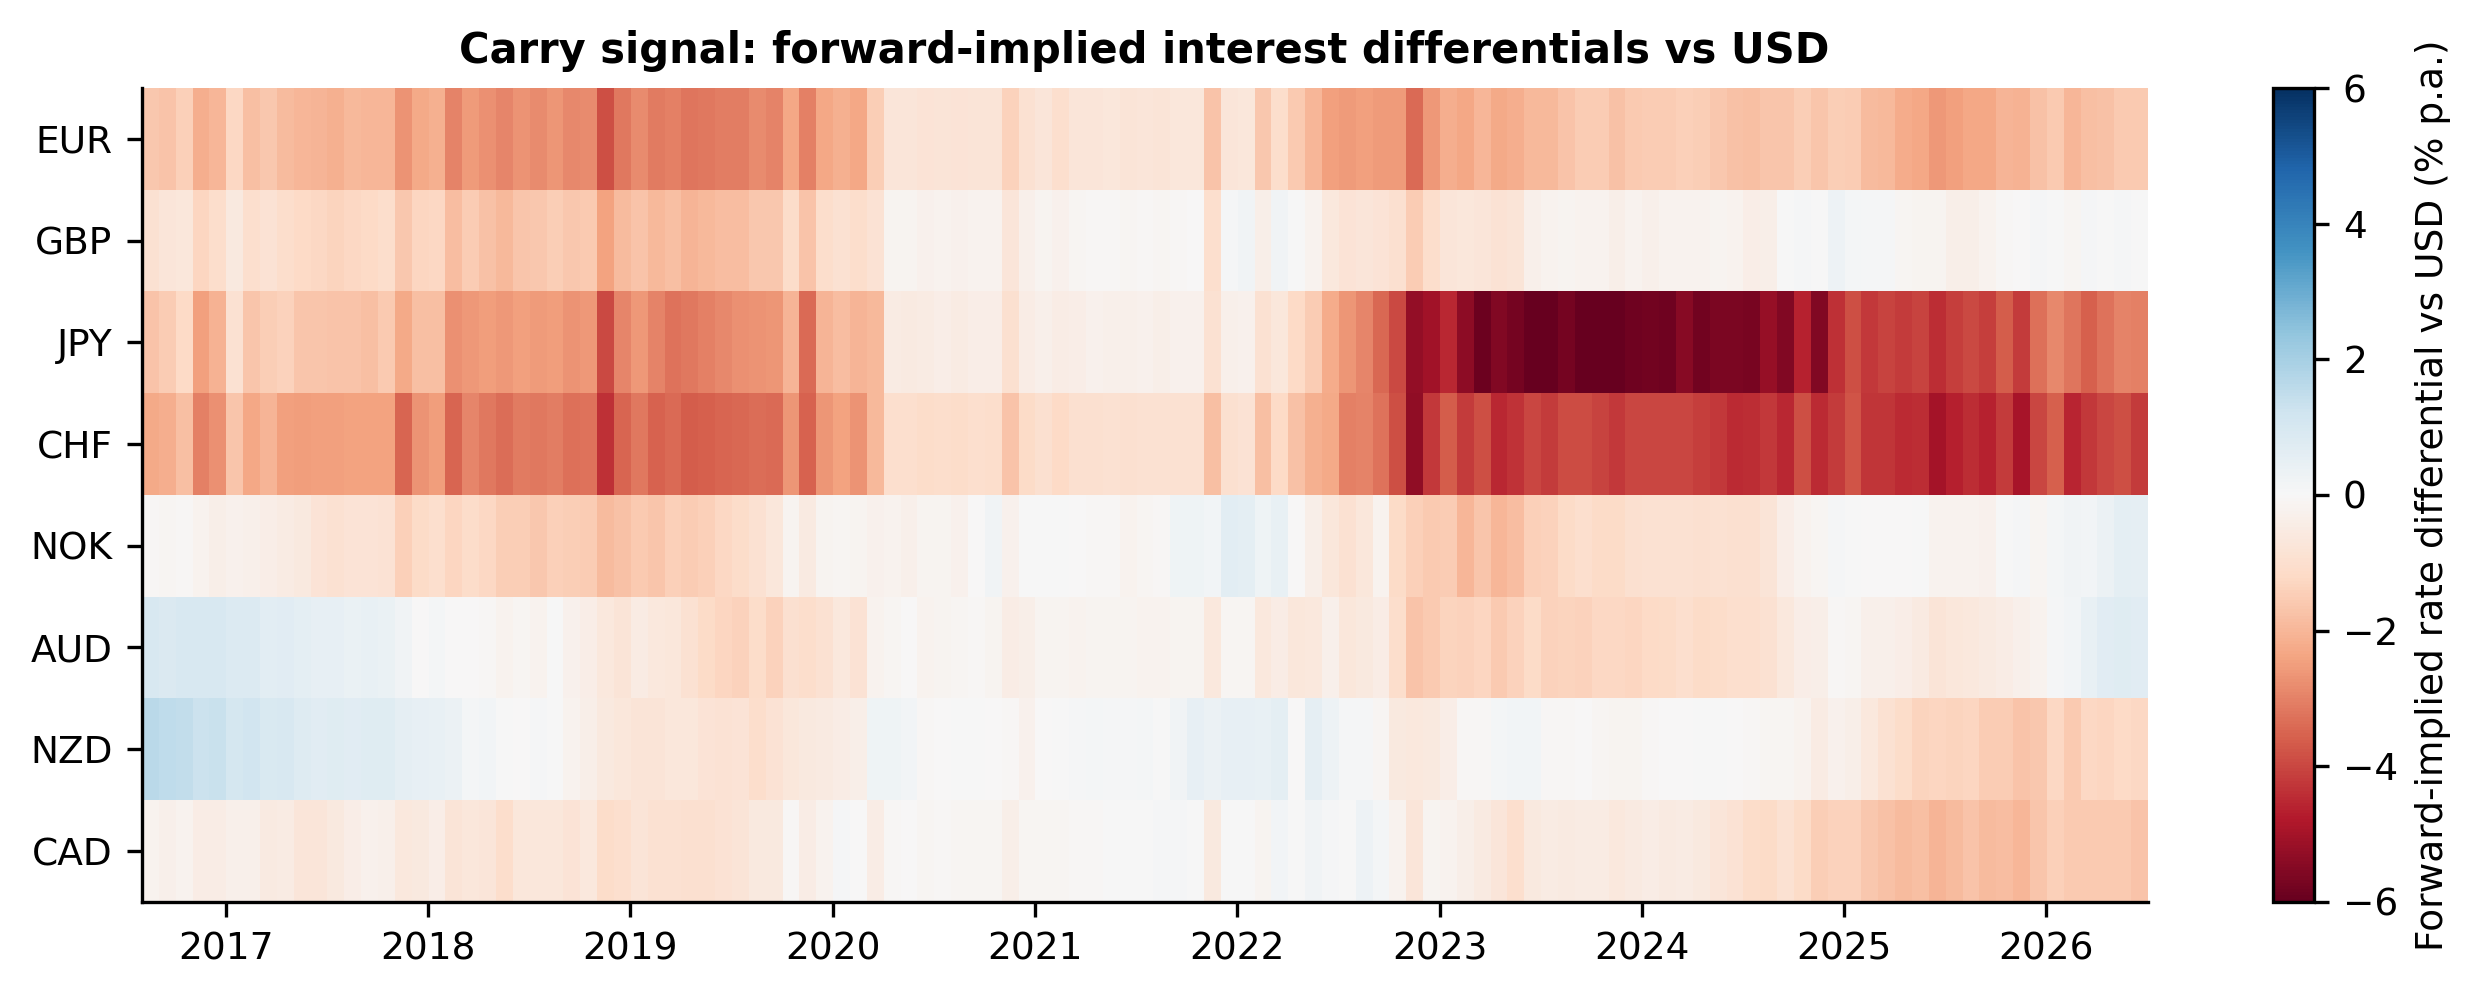
\includegraphics[width=0.95\textwidth]{figures/F10_differential_heatmap.png}\caption{Carry signal over time: forward-implied rate gap of each currency against USD (\% p.a.).}\label{fig:heat}\end{figure}

\begin{table}[!htbp]\centering\small
\caption{Bloomberg WIRP snapshot (17 August 2026) as a forward-looking check}\label{tab:wirp}
\begin{tabularx}{\textwidth}{lCCCCCC}
\toprule Currency & Current rate (\%) & Implied rate in about one year (\%) & Expected change (bp) & Forward rate gap now (\% p.a.) & Rank (WIRP) & Rank (forward) \\ \midrule
EUR & 2.19 & 2.78 & 59 & $-$1.55 & 6 & 5 \\
JPY & 0.98 & 1.80 & 82 & $-$3.39 & 7 & 7 \\
CAD & 2.28 & 2.90 & 62 & $-$1.56 & 5 & 6 \\
AUD & 4.35 & 4.79 & 44 & 0.64 & 1 & 1 \\
NOK & 4.25 & 4.48 & 23 & 0.49 & 2 & 2 \\
NZD & 2.50 & 3.38 & 88 & $-$1.12 & 4 & 4 \\
CHF & $-$0.06 & 0.20 & 25 & $-$4.28 & 8 & 8 \\
GBP & 3.73 & 4.35 & 62 & 0.04 & 3 & 3 \\
\bottomrule\end{tabularx}
\par\vspace{0.3em}\footnotesize\emph{USD: current implied rate 3.63\%, about 38 bp of hikes priced to July 2027. Rank correlation between the two rankings: 0.98.}
\end{table}

\subsection*{Annex B. Python program}
The whole analysis is run by one script, \texttt{src/carry\_project.py}. It reads the Bloomberg files in \texttt{data/} and writes
every table to \texttt{outputs/final/tables/} (also collected in \texttt{carry\_results.xlsx}) and every chart to
\texttt{outputs/final/figures/}. The steps are: (1) load spot and one-month forward rates and quote them as USD per currency;
(2) take month-end values and compute the forward-discount signal; (3) build the carry, momentum, static and dollar-basket
portfolios; (4) compute forward-based returns, the spot and carry parts, turnover and costs, and daily returns; (5) performance
statistics, sub-periods and VIX regimes; (6) UIP regressions; (7) worst months and days, drawdowns and the tail ratio;
(8) correlations, risk regressions and the Fama--MacBeth test; (9) the WIRP check and robustness tests. This paper is built by
\texttt{src/build\_latex.py}, which reads the same results file.
\subsection*{Annex C. Key events}

\begin{table}[H]\centering\small
\caption{Key market and policy events used in this paper}\label{tab:events}
\begin{tabularx}{\textwidth}{llY}
\toprule Date & Currencies & Event \\ \midrule
2016-11-08 & USD, JPY & US election: dollar and US yields rise, yen falls \\
2016-12-14 & USD & Fed hikes to 0.50--0.75\%; start of the 2017--18 hiking cycle \\
2018-02-05 & All & VIX spike (``Volmageddon''); carry $-$2.8\% in February 2018 \\
2018-07-06 & AUD, NZD & First US tariffs on China; trade war hits AUD and NZD \\
2018-12-19 & USD & Fed hikes to 2.25--2.50\%; late-2018 sell-off \\
2019-01-03 & JPY, AUD & Yen flash crash: AUD/JPY falls about 7\% in minutes \\
2019-08-05 & JPY, AUD & Chinese yuan breaks 7 per dollar; US calls China a currency manipulator \\
2020-03-09 & NOK, CAD & Saudi--Russia oil price war; stock crash \\
2020-03-15 & All & Fed cuts to zero; dollar swap lines to other central banks \\
2020-11-09 & All & Vaccine news; risk rally (carry $+$4.2\% in November 2020) \\
2021-11-26 & NOK, CAD & Omicron variant; oil sell-off \\
2022-02-24 & EUR, NOK & Russia invades Ukraine; energy shock \\
2022-09-21/23 & USD, GBP, JPY & Fed $+$75 bp; UK mini-budget; Japan buys yen (22 Sep) \\
2022-11-10 & USD & Soft US inflation data: largest one-day dollar fall since 2009 \\
2022-12-20 & JPY & Bank of Japan widens its bond-yield band; yen jumps \\
2023-03-10/19 & CHF, JPY & Silicon Valley Bank fails; UBS takes over Credit Suisse \\
2024-03-19 & JPY & Bank of Japan ends negative rates \\
2024-07-11/31 & JPY & Japan buys yen; BoJ hikes to 0.25\%; yen-carry unwind starts \\
2024-08-05 & JPY, all & Global carry crash: Nikkei $-$12.4\% \\
2025-04-02 & All & US ``Liberation Day'' tariffs; 90-day pause on 9 April \\
2025-12-19 & JPY & Bank of Japan hikes to 0.75\% \\
2026-02-28 & NOK, CAD, JPY & US--Israel strikes on Iran; Strait of Hormuz closed; oil above \$100 \\
2026-02 to 05 & AUD & RBA hikes three times, 3.60\% to 4.35\% \\
2026-04-28 & JPY & Japan starts record yen buying (\textyen 11.7tn, to 27 May) \\
2026-06-11/16 & EUR, JPY & ECB hikes to 2.25\%; Bank of Japan hikes to 1.00\% \\
\bottomrule\end{tabularx}
\par\vspace{0.3em}\footnotesize\emph{Full list of about 370 events: \texttt{data/macro\_event\_log.xlsx}.}
\end{table}

\subsection*{Annex D. Bloomberg functions}
\begin{table}[H]\centering\small
\caption{Bloomberg functions used}\label{tab:bbg}
\begin{tabularx}{\textwidth}{lYY}
\toprule Function & What it gives & How it is used \\ \midrule
GP & Daily spot rates for the 8 pairs; S\&P 500 and VIX & All returns, regimes and correlations \\
FRD & One-month forward points & Carry signal and forward-based returns \\
WIRP & Market-implied central-bank rate paths (17 Aug 2026) & Forward-looking check (Table~\ref{tab:wirp}) \\
FXIP & Forward points, overnight to six months (bid/ask) & Roll-cost estimate; positioning data not available \\
CORR & Rolling correlation of carry with SPX and VIX & Check Figure~\ref{fig:roll} on the terminal (252-day window) \\
REGR & Regression of carry on SPX and VIX change & Check Table~\ref{tab:risk} on the terminal \\
BTST & Strategy backtest & Optional check of Table~\ref{tab:perf} \\
\bottomrule\end{tabularx}
\end{table}

\end{document}